\documentclass[12pt,a4paper]{report}
\usepackage[spanish]{babel}
\usepackage[utf8]{inputenc}
\usepackage[T1]{fontenc}
\usepackage[margin=3cm]{geometry}
\usepackage{setspace}
\usepackage{booktabs}
\usepackage{longtable}
\usepackage{enumitem}
\usepackage{graphicx}
\usepackage{float}
\usepackage{caption}
\usepackage{subcaption}
\usepackage{amsmath}
\usepackage{listings}
\usepackage{xcolor}
\usepackage{csquotes}
\usepackage[colorlinks=true, linkcolor=blue, urlcolor=blue, citecolor=blue]{hyperref}
\usepackage[backend=biber, style=ieee, doi=true, url=true]{biblatex}
\addbibresource{refs.bib}
% Todos los captions de figuras/tablas del informe estan en ingles (P7);
% \figurename/\tablename de babel[spanish] seguian imprimiendo "Figura"/
% "Tabla" delante de esos captions en ingles. babel fija esos nombres al
% principio de \begin{document} (\selectlanguage), asi que un
% \renewcommand en el preambulo se sobreescribe; se usa \AtBeginDocument
% para que el nuestro se aplique despues. Se fuerza el rotulo a ingles
% para que coincida con el idioma real del contenido, igual que ya
% ocurre con "Listing" (paquete listings, no afectado por babel).
\AtBeginDocument{%
  \renewcommand{\figurename}{Figure}%
  \renewcommand{\tablename}{Table}%
}
\setstretch{1.5}
\setlength{\parindent}{1.5cm}
\setlength{\parskip}{6pt}

\lstset{
  basicstyle=\ttfamily\small,
  breaklines=true,
  frame=single,
  backgroundcolor=\color{gray!5},
  numbers=left,
  numberstyle=\tiny\color{gray},
  keywordstyle=\color{blue!70!black},
  commentstyle=\color{green!50!black},
  stringstyle=\color{red!60!black}
}

\begin{document}

% --- Portada ---
\begin{titlepage}
\centering
\vspace*{0.6cm}

{\Large UNIVERSIDAD TÉCNICA ESTATAL DE QUEVEDO}\\[0.2cm]
{\Large FACULTAD DE CIENCIAS DE LA COMPUTACIÓN}\\[0.2cm]
{\Large CARRERA DE INGENIERÍA DE SOFTWARE}\\[0.4cm]
{\large ASIGNATURA: APLICACIONES WEB}\\[0.2cm]
{\large CURSO: 5TO SOFTWARE ``A''}\\[1.2cm]

{\LARGE \textbf{Sistema de Gestión de Recursos Operativos,}}\\[0.2cm]
{\LARGE \textbf{Administrativos y de Seguridad para}}\\[0.2cm]
{\LARGE \textbf{Cooperativas de Transporte (SGROAS)}}\\[0.6cm]
{\large Informe del Proyecto Fin de Curso --- Versión 1.1.0 --- Entrega Final}\\[0.4cm]
{\small \texttt{\href{https://github.com/Alxjandr07/SGROAS-ProyectoAppWeb.git}{https://github.com/Alxjandr07/SGROAS-ProyectoAppWeb.git}}}\\[0.2cm]
{\small URL pública: \texttt{\href{https://sgroas-backend.onrender.com}{https://sgroas-backend.onrender.com}}}\\[0.2cm]
{\small Commit: \texttt{f7b9b72} $\vert$ DOI Software: 10.5281/zenodo.22522109 $\vert$ DOI Dataset: 10.5281/zenodo.21973297}\\[1.0cm]

\begin{minipage}{0.5\textwidth}
\centering
\textbf{ESTUDIANTES:}\\[0.4cm]
CASTRO ESPINOZA KEVIN MOISÉS\\
\textsc{ORCID: 0009-0004-4935-0439}\\[0.3cm]
ESCUDERO PLAZA MARÍA DEL ROSARIO\\
\textsc{ORCID: 0009-0007-3212-9924}\\[0.3cm]
TEJADA BAJAÑA LUIS ALEJANDRO\\
\textsc{ORCID: 0009-0006-2080-1798}
\end{minipage}
\hfill
\begin{minipage}{0.4\textwidth}
\centering
\textbf{DOCENTE:}\\[0.4cm]
ING. GUERRERO ULLOA GLEISTON CICERÓN\\[0.8cm]
\textbf{PERÍODO ACADÉMICO:}\\
2026--2027 PPA\\[0.8cm]
\textbf{FECHA:}\\
11 de septiembre de 2026
\end{minipage}

\vfill
\end{titlepage}


% --- Resumen (B.1) ---
\setcounter{page}{2}
\chapter*{Resumen}
\addcontentsline{toc}{chapter}{Resumen}

\textbf{Resumen (ES):}

El presente informe documenta el diseño, implementación y validación del Sistema de Gestión de Recursos Operativos, Administrativos y de Seguridad para Cooperativas de Transporte (SGROAS), aplicación web de tres capas desarrollada como Proyecto Fin de Curso en la Universidad Técnica Estatal de Quevedo. SGROAS gestiona recursos operativos, administrativos y de seguridad mediante arquitectura basada en Angular 20 (frontend), Spring Boot 3.5.x con Java 21 LTS (backend), PostgreSQL 16 y Redis 7. Ofrece autenticación stateless mediante JWT en cookie HttpOnly, CRUD completo para conductores, usuarios, rutas, vehículos, asignaciones e incidentes, ocho procedimientos almacenados/funciones SQL y reportes. La verificación se realizó mediante 293 pruebas JUnit 5 con cobertura JaCoCo del 95,49\% instrucciones / 88,38\% ramas / 95,94\% líneas (reporte completo, \texttt{jacoco.csv} versionado en \texttt{dataset/jacoco}), pruebas de carga k6 (3 corridas, 50 VUs, 30\,s) con media de medias 23,01\,ms IC95\% [-7,88; 53,91], p95 máximo 173,13\,ms (umbral 200\,ms, 0\% errores), análisis estático con SpotBugs 4.8.6 (0 hallazgos) y escaneo dinámico OWASP ZAP baseline (0 hallazgos altos, 2 medios de configuración CSP). Lighthouse reporta escritorio P=95 / A=91 / BP=92 / SEO=90 y móvil P=77 / A=91 / BP=92 / SEO=90 contra la URL pública. Los requisitos se especificaron conforme a ISO/IEC/IEEE 29148:2018 y se verificaron las 15 características del INCOSE v4. El SUS obtuvo media 68,5 (DT 13,98, IC95\% [60,76; 76,24], n=15, muestreo por conveniencia). El sistema se versiona como v1.0.0 con DOI Zenodo (software 10.5281/zenodo.22522109, dataset 10.5281/zenodo.21973297).

\textbf{Palabras clave:} ingeniería de requisitos, SRS, Spring Boot, Angular, JWT, PostgreSQL, OWASP, SpotBugs, ZAP, Lighthouse, JaCoCo, k6, SUS, ISO 29148, INCOSE, proyecto fin de curso.

\medskip

\textbf{Abstract (EN):}

This report documents the design, implementation and validation of the Operations, Administrative and Security Resource Management System for Transport Cooperatives (SGROAS), a three-tier web application developed as Final Course Project at the State Technical University of Quevedo. SGROAS manages operational, administrative and security resources through an architecture based on Angular 20 (frontend), Spring Boot 3.5.x with Java 21 LTS (backend), PostgreSQL 16 and Redis 7. It provides stateless JWT authentication in HttpOnly cookies, full CRUD for drivers, users, routes, vehicles, assignments and incidents, eight stored procedures/SQL functions and reports. Verification included 293 JUnit 5 tests with JaCoCo coverage of 95.49\% instructions / 88.38\% branches / 95.94\% lines (full report, \texttt{jacoco.csv} versioned in \texttt{dataset/jacoco}), k6 load tests (3 runs, 50 VUs, 30\,s) with mean-of-means 23.01\,ms 95\%CI [-7.88; 53.91], max p95 173.13\,ms (threshold 200\,ms, 0\% errors), static analysis with SpotBugs 4.8.6 (0 findings) and dynamic scanning with OWASP ZAP baseline (0 high, 2 medium CSP configuration findings). Lighthouse reports desktop P=95 / A=91 / BP=92 / SEO=90 and mobile P=77 / A=91 / BP=92 / SEO=90 against the public URL. Requirements follow ISO/IEC/IEEE 29148:2018 and all 15 INCOSE v4 characteristics were verified. SUS mean was 68.5 (SD 13.98, 95\%CI [60.76; 76.24], n=15, convenience sampling). The system is versioned as v1.0.0 with Zenodo DOI (software 10.5281/zenodo.22522109, dataset 10.5281/zenodo.21973297).

\textbf{Keywords:} requirements engineering, SRS, Spring Boot, Angular, JWT, PostgreSQL, OWASP, SpotBugs, ZAP, Lighthouse, JaCoCo, k6, SUS, ISO 29148, INCOSE, final course project.


% --- Índice general ---
\tableofcontents
\clearpage

% --- Índices de elementos (B.14) ---
\listoffigures
\clearpage
\listoftables
\clearpage
\lstlistoflistings
\clearpage

% --- Lista de siglas (B.3) ---
\input{siglas}
\clearpage

% --- Capítulo 1: Introducción (B.2, B.5) ---
\chapter{Introducción}
\label{cap:introduccion}

\section{Contexto y justificación}
\label{sec:contexto}

Las cooperativas de transporte urbano en Ecuador enfrentan desafíos significativos en la gestión de sus recursos operativos, administrativos y de seguridad. La planificación de rutas, la asignación de conductores y vehículos, el registro de incidentes y la generación de reportes se realizan frecuentemente mediante procesos manuales o semi-automatizados que dependen de hojas de cálculo, formatos en papel y sistemas de comunicación no estructurados \cite{sommerville2015}. Estas prácticas generan inconsistencias en los datos, demoras en la toma de decisiones y dificultades para el seguimiento del cumplimiento normativo.

El sector del transporte público en Ecuador mueve a más de 3 millones de pasajeros diarios en las principales ciudades, según datos del Ministerio de Transporte y Obras Públicas \cite{mtop2024}. La gestión ineficiente de la flota, las asignaciones de rutas sin herramientas digitales y la falta de un registro estructurado de incidentes de seguridad representan riesgos operativos que afectan directamente la calidad del servicio y la seguridad de los usuarios.

En este contexto, el desarrollo de un sistema de información web que centralice la gestión de los recursos de una cooperativa de transporte se convierte en una necesidad estratégica. SGROAS (Sistema de Gestión de Recursos Operativos, Administrativos y de Seguridad) fue concebido como una solución que integra las funcionalidades esenciales para la administración de conductores, usuarios, rutas, vehículos, asignaciones operativas e incidentes, proporcionando una plataforma unificada para el personal administrativo, operativo y de seguridad de la institución.

La motivación del proyecto se sustenta en tres pilares: (1) la necesidad real expresada por el personal de la cooperativa durante las entrevistas iniciales, (2) la oportunidad de aplicar los conocimientos adquiridos durante la carrera de Ingeniería de Software en un caso de uso real, y (3) la contribución al cuerpo de conocimiento en ingeniería de requisitos aplicada a sistemas de gestión de transporte en el contexto ecuatoriano.

\section{Descripción del problema}
\label{sec:problema}

La cooperativa de transporte objeto de estudio carece de un sistema integrado de información que soporte sus procesos operativos. Actualmente, la gestión de conductores se realiza mediante registros en hojas de cálculo que no garantizan la integridad de los datos. La asignación de rutas y vehículos se coordina por teléfono o mensajería instantánea, lo que dificulta el seguimiento y la auditoría. El registro de incidentes se realiza en formatos físicos que pueden extraviarse o ser incompletos. La generación de reportes operativos requiere la consolidación manual de datos de múltiples fuentes, proceso que consume tiempo y es propenso a errores.

Estos problemas se traducen en:
\begin{itemize}
  \item \textbf{Pérdida de información:} Registros en papel y hojas de cálculo no respaldadas generan pérdida de datos históricos.
  \item \textbf{Ineficiencia operativa:} La asignación manual de recursos consume tiempo valioso del personal coordinador.
  \item \textbf{Falta de trazabilidad:} No existe un registro estructurado de las decisiones operativas y los incidentes.
  \item \textbf{Limitaciones en reportes:} La ausencia de herramientas automatizadas dificulta la obtención de métricas para la toma de decisiones.
  \item \textbf{Riesgos de seguridad:} La gestión descentralizada de la información aumenta la exposición a incidentes de seguridad de datos.
\end{itemize}

\section{Preguntas de investigación}
\label{sec:preguntas}

El desarrollo de SGROAS se orienta a responder las siguientes preguntas de investigación:

\begin{enumerate}
  \item \textbf{RQ1:} ¿El acceso híbrido CRUD/ORM + procedimientos almacenados mantiene latencia aceptable bajo carga?

  \item \textbf{RQ2:} ¿El sistema mitiga los riesgos OWASP Top 10 con controles verificables?

  \item \textbf{RQ3:} ¿Qué nivel de usabilidad perciben los usuarios del sistema SGROAS?

  \item \textbf{RQ4:} ¿La interfaz web cumple estándares de rendimiento, accesibilidad y SEO según Lighthouse?
\end{enumerate}

\section{Objetivos}
\label{sec:objetivos}

\subsection{Objetivo general}

Diseñar, implementar y validar el Sistema de Gestión de Recursos Operativos, Administrativos y de Seguridad (SGROAS), una aplicación web de tres capas que gestione los recursos de una cooperativa de transporte, verificando la calidad de sus requisitos conforme a ISO/IEC/IEEE 29148:2018 y las 15 características del INCOSE Guide to Writing Requirements v4.

\subsection{Objetivos específicos}

\begin{enumerate}
  \item Especificar los requisitos funcionales y no funcionales del sistema SGROAS en un documento SRS conforme a ISO/IEC/IEEE 29148:2018, con trazabilidad completa hacia historias de usuario y casos de uso.

  \item Verificar las 15 características de calidad de requisitos (C1--C15) del INCOSE Guide to Writing Requirements v4 para cada requisito especificado.

  \item Implementar el backend del sistema utilizando Spring Boot 3.5.x con Java 21 LTS, PostgreSQL 16 y Redis 7, aplicando principios de arquitectura limpia y seguridad OWASP.

  \item Implementar el frontend del sistema utilizando Angular 20, con autenticación JWT en cookie HttpOnly y diseño responsivo.

  \item Ejecutar un conjunto de pruebas automatizadas que incluya pruebas unitarias, de integración y de carga, verificando cobertura mínima del 70\% y p95 menor a 200 ms.

  \item Realizar un escaneo de seguridad con OWASP ZAP y verificar el cumplimiento de las cabeceras HTTP de seguridad.

  \item Aplicar la prueba de System Usability Scale (SUS) con un mínimo de 15 participantes para evaluar la usabilidad percibida del sistema.
\end{enumerate}

\section{Contribuciones}
\label{sec:contribuciones}

Las contribuciones esperadas del proyecto SGROAS son:

\begin{enumerate}
  \item \textbf{Documento SRS v1.0.0:} Especificación completa de requisitos conforme a ISO/IEC/IEEE 29148:2018, con verificación INCOSE C1--C15, 50 requisitos (44 funcionales + 6 no funcionales) y trazabilidad completa.

  \item \textbf{Sistema funcional:} Aplicación web desplegable con Docker Compose, que integra autenticación JWT, CRUD completo para 6 entidades y ocho procedimientos almacenados/funciones SQL.

  \item \textbf{Evidencia de calidad:} 293 pruebas JUnit 5 con JaCoCo 95,49\% instrucciones / 88,38\% ramas / 95,94\% líneas (reporte completo), análisis estático SpotBugs 4.8.6 (0 hallazgos), escaneo OWASP ZAP baseline (0 High / 2 Med) y pruebas de carga k6 (3 corridas, media 23,01\,ms, p95 máx 173,13\,ms).

  \item \textbf{Validación de requisitos:} Checklist INCOSE verificando las 15 características de calidad para cada requisito del SRS, con evidencia de elicitación documentada.

  \item \textbf{Dataset reproducible:} Repositorio público en GitHub con código fuente, documentación, scripts de medición y datos semilla, archivado en Zenodo con DOI asignado.
\end{enumerate}

\section{Estructura del documento}
\label{sec:estructura}

El presente informe se organiza en los siguientes capítulos:

\begin{description}
  \item[Capítulo 1 — Introducción:] Contexto, justificación, descripción del problema, preguntas de investigación, objetivos y contribuciones (el presente capítulo).

  \item[Capítulo 2 — Marco Teórico:] Fundamentos teóricos y tecnológicos que sustentan el desarrollo del sistema: ISO/IEC/IEEE 29148:2018, INCOSE Guide, modelo C4, JWT, OWASP Top 10, Spring Boot, Angular, PostgreSQL y Redis.

  \item[Capítulo 3 — Trabajos Relacionados:] Revisión sistemática de literatura sobre sistemas de gestión de transporte y arquitecturas web, siguiendo PRISMA 2020.

  \item[Capítulo 4 — Ingeniería de Requisitos:] Proceso de elicitación, stakeholders, historias de usuario, casos de uso, matriz MoSCoW, matriz de trazabilidad y conformidad INCOSE.

  \item[Capítulo 5 — Materiales y Métodos:] Protocolo experimental, participantes SUS, métricas de evaluación (k6, JaCoCo, Lighthouse, ZAP, SUS) y amenazas a la validez.

  \item[Capítulo 6 — Diseño del Sistema y Arquitectura:] Arquitectura de tres capas, diagramas C4 (niveles 1--3), decisiones de diseño (ADR), diseño de base de datos y diseño de la API REST.

  \item[Capítulo 7 — Implementación:] Detalle de la implementación del backend (Spring Boot, PostgreSQL, Redis) y frontend (Angular), con listados de código representativos.

  \item[Capítulo 8 — Evaluación:] Resultados experimentales de rendimiento (k6), cobertura (JaCoCo), calidad web (Lighthouse), seguridad (ZAP) y usabilidad (SUS).

  \item[Capítulo 9 — Discusión:] Interpretación de resultados, comparación con trabajos relacionados y hallazgos inesperados.

  \item[Capítulo 10 — Amenazas a la Validez:] Análisis de las amenazas internas y externas a la validez del estudio experimental.

  \item[Capítulo 11 — Trabajo Futuro:] Líneas de mejora y extensión del sistema.

  \item[Capítulo 12 — Conclusiones:] Resumen de resultados, respuesta a las preguntas de investigación y limitaciones.
\end{description}


% --- Capítulo 2: Marco Teórico (B.4) ---
\chapter{Marco Teórico}
\label{cap:marco-teorico}

Este capítulo presenta los fundamentos teóricos y tecnológicos que sustentan el diseño e implementación del sistema SGROAS. Se organizan en cuatro áreas principales: ingeniería de requisitos, arquitectura de software, seguridad y tecnologías de implementación.

\section{Ingeniería de requisitos}
\label{sec:req-theory}

\subsection{ISO/IEC/IEEE 29148:2018}
\label{sec:iso29148}

La norma ISO/IEC/IEEE 29148:2018 \cite{iso29148} establece los procesos y productos asociados con la ingeniería de requisitos de software. Define un SRS (Software Requirements Specification) como el documento que captura los requisitos de software de un sistema, incluyendo sus requisitos funcionales, no funcionales y de interfaz.

Las características clave de un SRS conforme a esta norma son:
\begin{itemize}
  \item \textbf{Unambiguous:} Cada requisito se expresa de manera que solo admite una interpretación.
  \item \textbf{Complete:} El SRS incluye todos los requisitos significativos (funcionales, no funcionales y de diseño).
  \item \textbf{Consistent:} Los requisitos no contradictorios entre sí.
  \item \textbf{Verifiable:} Cada requisito puede verificarse mediante una técnica de verificación definida.
  \item \textbf{Traceable:} Cada requisito es rastreable hacia su origen y hacia los elementos de diseño.
\end{itemize}

SGROAS adopta la estructura de SRS recomendada por ISO/IEC/IEEE 29148:2018, organizando los requisitos en tres categorías: funcionales (REQ-F), no funcionales (REQ-NF) y de interfaz externa (REQ-IF). Cada requisito incluye su identificador, tipo, prioridad MoSCoW, justificación (rationale), enunciado, criterio de aceptación, método de verificación y trazabilidad.

\subsection{INCOSE Guide to Writing Requirements v4}
\label{sec:incose}

El INCOSE (International Council on Systems Engineering) publica la guía ``Guide to Writing Requirements'' \cite{incose}, que define 15 características de calidad para requisitos individuales y conjuntos de requisitos. Estas características se organizan en dos grupos:

\textbf{Características individuales (C1--C9):}
\begin{enumerate}
  \item[C1.] \textbf{Necessary:} El requisito es necesario para cumplir el objetivo del sistema.
  \item[C2.] \textbf{Appropriate:} El requisito es apropiado para el nivel de abstracción al que pertenece.
  \item[C3.] \textbf{Unambiguous:} El requisito se expresa de manera clara y sin ambigüedad.
  \item[C4.] \textbf{Complete:} El requisito contiene toda la información necesaria.
  \item[C5.] \textbf{Singular:} El requisito expresa un solo concepto.
  \item[C6.] \textbf{Feasible:} El requisito es factible de implementar.
  \item[C7.] \textbf{Verifiable:} El requisito puede verificarse mediante una técnica definida.
  \item[C8.] \textbf{Correct:} El requisito refleja la necesidad real del stakeholder.
  \item[C9.] \textbf{Conforming:} El requisito sigue las convenciones de formato establecidas.
\end{enumerate}

\textbf{Características del conjunto (C10--C15):}
\begin{enumerate}
  \item[C10.] \textbf{Complete (set):} El conjunto contiene todos los requisitos necesarios.
  \item[C11.] \textbf{Consistent (set):} Los requisitos no se contradicen entre sí.
  \item[C12.] \textbf{Comprehensible:} El conjunto es comprensible para los stakeholders.
  \item[C13.] \textbf{Able to be validated:} El conjunto puede validarse contra las necesidades del usuario.
  \item[C14.] \textbf{Trazable:} Cada requisito es rastreable hacia su origen.
  \item[C15.] \textbf{Unico (set):} Cada requisito es único dentro del conjunto.
\end{enumerate}

SGROAS verifica las 15 características C1--C15 para cada uno de sus 50 requisitos en el checklist \texttt{docs/checklists/incose2023-req.md}.

\subsection{Historias de usuario y casos de uso}
\label{sec:hu-cu}

Las historias de usuario, introducidas por Cohn \cite{cohn2004}, son una técnica de captura de requisitos que se expresa en el formato: ``Como [rol], quiero [acción] para [valor]''. Cada historia se valida mediante criterios de aceptación en formato Gherkin (Given/When/Then). Las historias de usuario se evalúan con los criterios INVEST: Independent, Negotiable, Valuable, Estimable, Small y Testable.

Los casos de uso, formalizados por Cockburn \cite{cockburn2001}, describen las interacciones entre actores y el sistema para lograr un objetivo. Se organizan en niveles de detalle (Cockburn 1--4) que van desde el objetivo del usuario hasta el flujo paso a paso. Los casos de uso incluyen escenarios principales de éxito y extensiones (casos de excepción).

SGROAS combina ambas técnicas: 8 historias de usuario con criterios Gherkin (formato Connextra) y 6 casos de uso en formato Cockburn niveles 1--4, garantizando cobertura completa de los requisitos funcionales.

\subsection{Matriz MoSCoW}
\label{sec:moscow}

La técnica MoSCoW \cite{wiegers2013} prioriza los requisitos en cuatro categorías:
\begin{itemize}
  \item \textbf{Must:} Requisito obligatorio; el sistema no es útil sin él.
  \item \textbf{Should:} Requisito importante; se incluye si hay recursos disponibles.
  \item \textbf{Could:} Requisito deseable; se incluye si sobra tiempo.
  \item \textbf{Won't:} Requisito pospuesto a futuras versiones.
\end{itemize}

SGROAS clasifica 44 requisitos como Must (88\%) y 6 como Should (12\%), reflejando un sistema con funcionalidad central consolidada y reportes como capacidades complementarias.

\section{Arquitectura de software}
\label{sec:architecture-theory}

\subsection{Modelo C4}
\label{sec:c4}

El modelo C4 \cite{c4model} es una técnica de documentación arquitectónica que describe un sistema en cuatro niveles de abstracción:
\begin{enumerate}
  \item \textbf{Contexto (nivel 1):} Describe el sistema en su entorno, mostrando actores y sistemas externos.
  \item \textbf{Contenedores (nivel 2):} Muestra las aplicaciones y bases de datos que componen el sistema.
  \item \textbf{Componentes (nivel 3):} Detalla los componentes internos de cada contenedor.
  \item \textbf{Código (nivel 4):} Describe la estructura de clases o módulos (opcional).
\end{enumerate}

SGROAS documenta su arquitectura en los niveles 1--3 mediante diagramas DSL (Domain Specific Language) generados con Structurizr, ubicados en \texttt{docs/arquitectura/}. Los diagramas C4 proporcionan una visión escalonada que facilita la comprensión de la arquitectura para diferentes audiencias.

\subsection{Arquitectura de tres capas}
\label{sec:three-tier}

La arquitectura de tres capas separa la presentación (frontend), la lógica de negocio (backend) y el almacenamiento de datos (base de datos) en capas independientes \cite{martin2017}. SGROAS implementa esta arquitectura con:
\begin{itemize}
  \item \textbf{Capa de presentación:} Angular 20, que consume la API REST del backend.
  \item \textbf{Capa de lógica de negocio:} Spring Boot 3.2.x con Java 21 LTS, que implementa los controladores, servicios y repositorios.
  \item \textbf{Capa de datos:} PostgreSQL 16 para persistencia y Redis 7 como caché distribuida.
\end{itemize}

\section{Seguridad}
\label{sec:security-theory}

\subsection{OWASP Top 10:2021}
\label{sec:owasp}

El OWASP (Open Worldwide Application Security Project) publica periódicamente la lista de los 10 riesgos de seguridad más críticos en aplicaciones web \cite{owasp}. Los riesgos más relevantes para SGROAS son:

\begin{description}
  \item[A01 — Broken Access Control:] El mecanismo de autenticación JWT en cookie HttpOnly + Secure + SameSite=Strict, combinado con la autorización por rol, mitiga este riesgo.
  \item[A02 — Cryptographic Failures:] TLS v1.3 en producción y cifrado de contraseñas con bcrypt mitigan este riesgo.
  \item[A03 — Injection:] El uso de JPA con consultas parametrizadas y la prohibición de SQL dinámico en procedimientos almacenados mitigan este riesgo.
  \item[A05 — Security Misconfiguration:] Las cabeceras HTTP de seguridad (HSTS, CSP, X-Frame-Options, X-Content-Type-Options) mitigan este riesgo.
  \item[A07 — Identification and Authentication Failures:] El rate limiting en login (6 intentos, respuesta 429) mitiga este riesgo.
\end{description}

\subsection{JWT (RFC 7519)}
\label{sec:jwt}

JSON Web Token (JWT) \cite{rfc7519} es un estándar para la representación segura de afirmaciones entre dos partes. Un JWT se compone de tres partes: header (algoritmo y tipo), payload (claims) y signature (firma). SGROAS genera JWTs con 7 claims: \texttt{iss} (emisor), \texttt{sub} (sujeto), \texttt{aud} (audiencia), \texttt{exp} (expiración), \texttt{nbf} (no antes de), \texttt{iat} (emitido en) y \texttt{jti} (identificador único). El JWT se almacena en una cookie HttpOnly + Secure + SameSite=Strict, evitando el acceso desde JavaScript del navegador.

\subsection{ProblemDetails (RFC 7807)}
\label{sec:rfc7807}

El estándar RFC 7807 \cite{rfc7807} define un formato uniforme para los errores en APIs HTTP. SGROAS implementa ProblemDetails en todas las respuestas de error, incluyendo los campos \texttt{type}, \texttt{title}, \texttt{status}, \texttt{detail} e \texttt{instance}. Esto garantiza que los clientes puedan manejar los errores de manera consistente y automatizada.

\section{Tecnologías de implementación}
\label{sec:tech}

\subsection{Spring Boot 3.2.x con Java 21 LTS}
\label{sec:spring}

Spring Boot \cite{springboot} es un framework que simplifica la creación de aplicaciones basadas en Spring. SGROAS utiliza Spring Boot 3.2.x con Java 21 LTS (Long Term Support), aprovechando:
\begin{itemize}
  \item Spring Data JPA con Hibernate para el mapeo objeto-relacional (ORM).
  \item Spring Security para la autenticación y autorización.
  \item Spring Cache con Redis para la caché distribuida.
  \item Flyway para las migraciones de base de datos.
  \item SpringDoc OpenAPI para la documentación automática de la API.
\end{itemize}

\subsection{Angular 20}
\label{sec:angular}

Angular \cite{angular} es un framework de desarrollo frontend mantenido por Google. SGROAS utiliza Angular 20 con TypeScript, aprovechando:
\begin{itemize}
  \item Componentes y módulos para la organización del código.
  \item Servicios e inyección de dependencias para la comunicación con la API.
  \item Angular Router para la navegación entre vistas.
  \item HttpClient para las peticiones HTTP al backend.
\end{itemize}

\subsection{PostgreSQL 16}
\label{sec:postgresql}

PostgreSQL \cite{postgresql} es un sistema de gestión de bases de datos relacional de código abierto. SGROAS utiliza PostgreSQL 16 aprovechando:
\begin{itemize}
  \item Procedimientos almacenados para reportes y agregaciones complejas.
  \item Funciones SQL para estadísticas y métricas.
  \item Triggers para auditoría y validación de datos.
  \item Índices para optimización de consultas.
  \item Tipos enumerados para estados y categorías.
\end{itemize}

\subsection{Redis 7}
\label{sec:redis}

Redis \cite{redis} es un almacén de datos en memoria utilizado como caché distribuida. SGROAS emplea Redis para:
\begin{itemize}
  \item Caché del listado paginado de conductores con TTL configurable.
  \item Lista negra de tokens JWT revocados (JTI en logout).
  \item Rate limiting para el control de intentos de login.
\end{itemize}

\section{Estándares de calidad}
\label{sec:quality}

\subsection{ISO/IEC 25010:2011}
\label{sec:iso25010}

La norma ISO/IEC 25010:2011 \cite{iso25010} define un modelo de calidad del producto software con ocho características: adecuación funcional, eficiencia de desempeño, compatibilidad, usabilidad, fiabilidad, seguridad, mantenibilidad y portabilidad. SGROAS verifica explícitamente las siguientes características:
\begin{itemize}
  \item \textbf{Adecuación funcional:} El sistema cumple con los 44 requisitos funcionales especificados.
  \item \textbf{Eficiencia de desempeño:} El p95 del listado de conductores es de 173,13\,ms máx (media de medias 23,01\,ms IC95\% [-7,88;53,91], umbral 200\,ms, 0\% errores).
  \item \textbf{Seguridad:} Cabeceras HTTP de seguridad, JWT en cookie HttpOnly, rate limiting, parametrización de consultas.
  \item \textbf{Usabilidad:} SUS de 68,5 (DT 13,98, n=15).
\end{itemize}

\subsection{Métricas de calidad de código}
\label{sec:code-quality}

La calidad de código se mide mediante:
\begin{itemize}
  \item \textbf{Cobertura de pruebas (JaCoCo):} reporte completo 95,49\% instrucciones / 88,38\% ramas / 95,94\% líneas (datos reproducibles en \texttt{dataset/jacoco/jacoco.csv}).
  \item \textbf{Número de pruebas:} 293 pruebas JUnit 5 (unitarias e de integración).
  \item \textbf{Deuda técnica:} Verificación mediante el plugin de SonarQube en CI.
\end{itemize}


% --- Capítulo 3: Trabajos Relacionados (B.6) ---
\chapter{Trabajos Relacionados}
\label{cap:trabajos-relacionados}

Este capítulo presenta una revisión estructurada de trabajos previos sobre sistemas de gestión de transporte y arquitecturas web para aplicaciones de gestión de recursos. La búsqueda se documenta siguiendo la orientación metodológica de Kitchenham y Charters \cite{kitchenham2013} y se reporta con la disciplina de PRISMA 2020 \cite{prisma2021}.

\section{Estrategia de búsqueda}
\label{sec:estrategia-busqueda}

\subsection{Bases de datos consultadas}

Se consultaron las siguientes bases de datos: IEEE Xplore, ACM Digital Library, Scopus, ScienceDirect y Springer Link. La ventana temporal fue de 2018 a 2026, considerando trabajos de los últimos ocho años para capturar tanto soluciones consolidadas como tendencias recientes.

\subsection{Cadena de búsqueda}

La cadena de búsqueda combina sinónimos y operadores booleanos:

\begin{verbatim}
("transport management" OR "fleet management" OR "public transit")
AND ("web application" OR "web system" OR "information system")
AND ("Spring Boot" OR "Java" OR "Angular" OR "React" OR "PostgreSQL")
AND ("REST API" OR "microservices" OR "monolith")
\end{verbatim}

\subsection{Criterios de inclusión y exclusión}

\textbf{Inclusión:} (I1) Sistemas web de gestión de transporte o flota; (I2) Utilizan arquitectura de tres capas o similar; (I3) Incluyen evaluación empírica (rendimiento, usabilidad o seguridad); (I4) Publicados en conferencias o revistas del área de ingeniería de software.

\textbf{Exclusión:} (E1) Artículos de opinión o tutoriales sin evaluación; (E2) Sistemas móviles nativos sin componente web; (E3) Trabajos cuyo dominio no es transporte/gestión de flota; (E4) Artículos duplicados entre bases de datos.

\section{Diagrama de flujo PRISMA}
\label{sec:prisma}

El proceso de selección siguió las cuatro fases de PRISMA 2020 \cite{prisma2021}:

\begin{enumerate}
  \item \textbf{Identificación:} 142 registros identificados en las cinco bases de datos (IEEE Xplore: 38, ACM: 29, Scopus: 41, ScienceDirect: 22, Springer: 12).
  \item \textbf{Cribado:} 96 registros tras eliminación de duplicados (46 duplicados). Se revisaron títulos y resúmenes.
  \item \textbf{Elegibilidad:} 24 artículos recuperados en texto completo.
  \item \textbf{Incluidos:} 10 trabajos incluidos en la síntesis final tras aplicar criterios de inclusión/exclusión.
\end{enumerate}

Los motivos de exclusión de los 14 artículos eliminados en la fase de elegibilidad fueron: sin evaluación empírica (6), dominio no relacionado con transporte (4), sistema móvil sin componente web (2) y publicación duplicada (2).

\section{Síntesis de trabajos incluidos}
\label{sec:sintesis-trabajos}

Table~\ref{tab:trabajos-relacionados} resume los 10 trabajos incluidos, comparados con SGROAS en las dimensiones relevantes.

\begin{longtable}{@{}p{2.2cm}p{1cm}p{1.8cm}p{1.8cm}p{1.5cm}p{1.5cm}p{2cm}@{}}
\caption{Related works and comparison with SGROAS.}
\label{tab:trabajos-relacionados}\\
\toprule
\textbf{Referencia} & \textbf{Año} & \textbf{Dominio} & \textbf{Tecnologías} & \textbf{Arq.} & \textbf{Evaluación} & \textbf{Diferencia con SGROAS} \\
\midrule
\endfirsthead
\toprule
\textbf{Referencia} & \textbf{Año} & \textbf{Dominio} & \textbf{Tecnologías} & \textbf{Arq.} & \textbf{Evaluación} & \textbf{Diferencia con SGROAS} \\
\midrule
\endhead
\cite{alshuqayran2016} & 2016 & Transporte público & Java, REST & Microservicios & Mapeo sistemático & Enfoque en microservicios; SGROAS usa monolito \\ \midrule
\cite{taibi2018} & 2018 & Microservicios & Varios & Microservicios & Bad smells & Catálogo de deuda técnica; SGROAS evalúa propiedades \\ \midrule
\cite{soldani2018} & 2018 & Microservicios & Varios & Microservicios & Revisión grey & Pains/gains de microservicios; SGROAS valida monolito \\ \midrule
\cite{waseem2021} & 2021 & Microservicios & Varios & Microservicios & Encuesta & Prácticas de practitioner; SGROAS aplica DSR \\ \midrule
\cite{jiang2015} & 2015 & Carga web & Varios & Varios & Survey & Metodología de load testing; SGROAS usa k6 con IC 95\% \\ \midrule
\cite{jiang2009} & 2009 & Rendimiento & Java EE & 3 capas & Experimento & Análisis automatizado; SGROAS incluye contraste no paramétrico \\ \midrule
\cite{inozemtseva2014} & 2014 & Cobertura & Varios & Varios & Experimento & Cobertura vs efectividad; SGROAS combina con integración \\ \midrule
\cite{brooke1996} & 1996 & Usabilidad & Varios & Varios & SUS & Instrumento estándar; SGROAS aplica con escala adjetiva \\ \midrule
\cite{pautasso2008} & 2008 & Web services & REST vs SOAP & REST & Comparación & REST vs big web services; SGROAS adopta REST \\ \midrule
\cite{fielding2002} & 2002 & Web & HTTP & REST & Diseño & Fundamentos REST; SGROAS sigue principios REST \\
\bottomrule
\end{longtable}

\section{Brecha identificada}
\label{sec:brecha}

Los trabajos revisados abordan dominios relacionados con transporte, arquitecturas web y evaluación empírica, pero presentan las siguientes limitaciones que SGROAS busca contribuir a cubrir:

\begin{enumerate}
  \item \textbf{Falta de sistemas web completos para cooperativas de transporte ecuatoriano:} la mayoría de trabajos se enfocan en microservicios \cite{alshuqayran2016,soldani2018,taibi2018,waseem2021} o en dominios distintos al transporte público en contextos latinoamericanos. SGROAS aporta un sistema completo (backend + frontend + BD) documentado con SRS ISO/IEC/IEEE 29148:2018.

  \item \textbf{Evaluación empírica incompleta:} varios trabajos reportan métricas de rendimiento sin intervalo de confianza \cite{jiang2009} o sin contraste estadístico formal. SGROAS incluye media, DT, IC 95\%, test inferencial (Wilcoxon) y tamaño de efecto (Cliff delta), siguiendo la guía de experimentación de Wohlin et al. \cite{wohlin2012}.

  \item \textbf{Ausencia de estrategia híbrida de acceso a datos documentada:} los trabajos de arquitectura web \cite{pautasso2008,fielding2002} describen patrones REST pero no documentan la separación CRUD-ORM / stored procedures con evidencia de seguridad (análisis estático de SQL dinámico). SGROAS documenta esta decisión formalmente (ADR-006) y la audita con scripts reproducibles.

  \item \textbf{Falta de reproducibilidad completa:} la mayoría de trabajos no publican datos crudos ni scripts de análisis. SGROAS cumple los principios FAIR \cite{wilkinson2016} con datos versionados, scripts reproducibles y DOI de Zenodo.
\end{enumerate}


% --- Capítulo 4: Ingeniería de Requisitos (B.7) ---
\chapter{Ingeniería de Requisitos}
\label{cap:req-engineering}

Este capítulo describe el proceso completo de ingeniería de requisitos aplicado al sistema SGROAS, desde la identificación de stakeholders hasta la verificación de conformidad con las características INCOSE. El proceso se ejecutó de manera iterativa entre mayo y agosto de 2026, siguiendo las recomendaciones de ISO/IEC/IEEE 29148:2018 \cite{iso29148} y el INCOSE Guide to Writing Requirements v4 \cite{incose}.

\section{Stakeholders}
\label{sec:stakeholders}

La identificación de stakeholders se realizó mediante revisión documental del organigrama de la cooperativa y entrevistas iniciales con el personal directivo. Se clasificaron en seis categorías:

\begin{longtable}{@{}p{3.5cm}p{3cm}p{8cm}@{}}
\toprule
\textbf{Stakeholder} & \textbf{Rol en el proyecto} & \textbf{Necesidades principales} \\
\midrule
\endhead
Administrador del sistema & Usuario final, decisor & Gestión de usuarios, control de acceso, reportes ejecutivos \\
Coordinador de operaciones & Usuario final & Gestión de conductores, rutas, vehículos, asignaciones \\
Personal de seguridad & Usuario final & Registro y consulta de incidentes \\
Conductores & Usuarios indirectos & Información de rutas asignadas \\
Director de la cooperativa & Patrocinador & Reportes ejecutivos, estadísticas \\
Equipo de desarrollo (PFC) & Desarrolladores & Requisitos claros, trazabilidad, calidad \\
\bottomrule
\end{longtable}

Los stakeholders se priorizaron según su nivel de influencia e interés, identificando al administrador y al coordinador como los usuarios primarios con mayor impacto en la definición de requisitos.

\section{Proceso de elicitación}
\label{sec:elicitation}

Se aplicaron cinco técnicas de elicitación de requisitos, documentadas en \texttt{docs/requisitos/elicitacion/elicitation-evidence.md}:

\begin{enumerate}
  \item \textbf{Entrevista semiestructurada (10 mayo 2026):} Se entrevistó al coordinador de operaciones y al administrador del sistema. Se identificaron los requisitos iniciales: autenticación, CRUD de conductores y reportes básicos. Las entrevistas duraron aproximadamente 90 minutos cada una y se grabaron con consentimiento del participante.

  \item \textbf{Observación directa (15 mayo 2026):} Se observaron los flujos operativos del personal de seguridad y los conductores durante una jornada laboral. Se documentaron los procesos de asignación de rutas y registro de incidentes en formato físico, identificando puntos de mejora y requisitos no expresados.

  \item \textbf{Cuestionario online (20 mayo 2026):} Se distribuyó un cuestionario Google Forms a 12 empleados de la cooperativa. El cuestionario incluyó preguntas de priorización MoSCoW para funcionalidades candidatas y una escala de satisfacción percibida. Se obtuvieron 10 respuestas completas.

  \item \textbf{Revisión de documentación existente (25 mayo 2026):} Se analizaron las políticas de seguridad informática, los formatos de incidentes en papel, el organigrama institucional y los flujos operativos documentados. Esta técnica proporcionó contexto para la definición de restricciones y supuestos.

  \item \textbf{Taller JAD (1 junio 2026):} Se realizó un taller conjunto (Joint Application Design) con el coordinador, el personal de seguridad y el administrador. Se validaron las historias de usuario, los casos de uso y las prioridades MoSCoW. El taller duró 3 horas y se documentó en acta.
\end{enumerate}

\section{Historias de usuario}
\label{sec:hu}

Se definieron 8 historias de usuario en formato Connextra (``Como [rol], quiero [acción] para [valor]''), cada una con criterios de aceptación en formato Gherkin (Given/When/Then). Las historias se evaluaron con los criterios INVEST de Cohn \cite{cohn2004}.

\begin{longtable}{@{}p{2cm}p{3cm}p{4cm}p{4cm}@{}}
\toprule
\textbf{ID} & \textbf{Rol} & \textbf{Historia} & \textbf{Criterios Gherkin} \\
\midrule
\endhead
HU-001 & Admin/Coord/Seg & Iniciar sesión en el sistema & 3 escenarios (éxito, credenciales inválidas, sin autenticación) \\
HU-002 & Coord/Admin & Gestionar conductores (CRUD) & 4 escenarios (crear, consultar, actualizar, eliminar) \\
HU-003 & Admin & Gestionar usuarios del sistema (CRUD) & 4 escenarios (crear, consultar, actualizar, eliminar) \\
HU-004 & Coord/Admin & Gestionar rutas de transporte (CRUD) & 6 escenarios (crear, consultar, actualizar, eliminar, no encontrado, validación) \\
HU-005 & Coord/Admin & Gestionar vehículos (CRUD) & 5 escenarios (registrar, listar, mantener, actualizar, desactivar) \\
HU-006 & Coordinador & Asignar conductores y vehículos a rutas & 4 escenarios (crear, consultar activas, conflicto, listar) \\
HU-007 & Seguridad & Registrar y consultar incidentes & 5 escenarios (registrar, por rango, por gravedad, listar, no encontrado) \\
HU-008 & Admin/Coord & Generar reportes y estadísticas & 4 escenarios (rendimiento, generales, licencias, acceso no autorizado) \\
\bottomrule
\end{longtable}

Las historias HU-001 a HU-003 se heredaron de la Entrega 1B y se mantuvieron sin cambios. Las historias HU-004 a HU-008 se definieron para la Entrega Final, cubriendo las funcionalidades nuevas del sistema.

\section{Casos de uso}
\label{sec:cu}

Se definieron 6 casos de uso en formato Cockburn \cite{cockburn2001} con cuatro niveles de detalle (Cockburn 1--4). Cada caso incluye actor principal, actor secundario, precondiciones, postcondiciones, escenario principal de éxito y extensiones:

\begin{longtable}{@{}p{1.5cm}p{3cm}p{3cm}p{6cm}@{}}
\toprule
\textbf{ID} & \textbf{Nombre} & \textbf{Actor principal} & \textbf{Descripción} \\
\midrule
\endhead
CU-001 & Inicio de sesión & Usuario & Autenticación con JWT en cookie HttpOnly \\
CU-002 & Gestión de conductores & Coordinador & CRUD completo de conductores con paginación \\
CU-003 & Gestión de usuarios & Administrador & CRUD completo de usuarios con control de roles \\
CU-004 & Gestión de rutas & Coordinador & CRUD de rutas con validación de distancia \\
CU-005 & Gestión de vehículos & Coordinador & CRUD de vehículos con control de placa única \\
CU-006 & Asignaciones e incidentes & Coord/Seguridad & Asignación de recursos y registro de incidentes \\
\bottomrule
\end{longtable}

Los casos de uso CU-001 a CU-003 se heredaron de entregas anteriores. Los casos CU-004 a CU-006 se definieron para la Entrega Final. Cada caso de uso se documentó en un archivo Markdown individual en \texttt{docs/requisitos/casos-de-uso/}.

\section{Priorización MoSCoW}
\label{sec:moscow-application}

Los 50 requisitos identificados se priorizaron mediante la técnica MoSCoW \cite{wiegers2013}, resultando en la distribución mostrada en Table~\ref{tab:moscow}:

\begin{table}[H]
\centering
\caption{Requirements distribution by MoSCoW priority}
\label{tab:moscow}
\begin{tabular}{lcc}
\toprule
\textbf{Prioridad} & \textbf{Cantidad} & \textbf{Porcentaje} \\
\midrule
Must & 44 & 88\% \\
Should & 6 & 12\% \\
Could & 0 & 0\% \\
Won't & 0 & 0\% \\
\midrule
\textbf{Total} & \textbf{50} & \textbf{100\%} \\
\bottomrule
\end{tabular}
\end{table}

La alta proporción de requisitos Must (88\%) refleja la naturaleza del sistema: SGROAS es una aplicación de gestión donde la funcionalidad central (CRUD, autenticación, seguridad) es indispensable. Los 6 requisitos Should corresponden a reportes y funciones SQL que complementan la funcionalidad principal.

\section{Matriz de trazabilidad}
\label{sec:traceability}

La matriz de trazabilidad (\texttt{docs/trazabilidad/matriz.csv}) conecta cada requisito con su historia de usuario, caso de uso, módulo de código, endpoint API, prueba automatizada, evidencia empírica y estado de verificación. La matriz cubre el 100\% de los requisitos y se valida automáticamente mediante \texttt{scripts/validate-traceability.sh} en el pipeline de CI.

La matriz incluye la columna \texttt{tipo\_acceso} que clasifica cada requisito según su mecanismo de acceso a datos:
\begin{itemize}
  \item \textbf{CRUD-ORM:} Operaciones CRUD mapeadas mediante JPA/Hibernate.
  \item \textbf{SP:} Procedimientos almacenados en PostgreSQL.
  \item \textbf{FN:} Funciones SQL en PostgreSQL.
\end{itemize}

\section{Conformidad INCOSE}
\label{sec:incose-compliance}

Cada uno de los 50 requisitos del SRS v1.0.0 se verificó contra las 15 características de calidad del INCOSE Guide to Writing Requirements v4 \cite{incose}. El checklist completo se encuentra en \texttt{docs/checklists/incose2023-req.md}.

Los resultados de la verificación se resumen en Table~\ref{tab:incose}:

\begin{table}[H]
\centering
\caption{INCOSE compliance summary C1--C15}
\label{tab:incose}
\begin{tabular}{lcc}
\toprule
\textbf{Resultado} & \textbf{Requisitos} & \textbf{Porcentaje} \\
\midrule
Sí en las 15 características & 18 de 20 & 90\% \\
Parcial en alguna característica & 2 de 20 & 10\% \\
\midrule
\textbf{Total} & \textbf{20} & \textbf{100\%} \\
\bottomrule
\end{tabular}
\end{table}

Los dos requisitos con verificación parcial son:
\begin{itemize}
  \item \textbf{REQ-NF-002 (Cifrado TLS):} Parcial en C3, C4, C7, C8 y C12. El enunciado declara TLS v1.3 pero el entorno de desarrollo opera en HTTP plano. Se aclaró que TLS aplica exclusivamente a producción.
  \item \textbf{REQ-NF-006 (Cobertura):} Parcial en C4. El umbral declarado (60\%) es obsoleto; se actualizó a 70\% para la Entrega Final.
\end{itemize}

\section{Gestión del cambio}
\label{sec:change-management}

Las modificaciones a los requisitos se registran en \texttt{docs/requisitos/CHANGELOG-REQ.md} siguiendo el formato Keep a Changelog. Las decisiones de diseño que afectan requisitos Must se documentan como ADR (Architecture Decision Records) en \texttt{docs/adr/} siguiendo la plantilla de Nygard \cite{nygard2017}. El repositorio contiene 6 ADRs que cubren las decisiones más significativas del sistema.

\section{Resumen de requisitos}
\label{sec:req-summary}

El SRS v1.0.0 de SGROAS contiene:
\begin{itemize}
  \item \textbf{44 requisitos funcionales} (REQ-F-001 a REQ-F-040, con agrupaciones): 14 de autenticación y CRUD de conductores/usuarios (heredados de entregas anteriores) + 30 nuevos para rutas, vehículos, asignaciones, incidentes y reportes.
  \item \textbf{6 requisitos no funcionales} (REQ-NF-001 a REQ-NF-010): seguridad HTTP, TLS, rendimiento, inyección, rate limiting, cobertura, OpenAPI, ProblemDetails, CORS por origen y CORS por rol.
  \item \textbf{8 historias de usuario} con criterios Gherkin (formato Connextra).
  \item \textbf{6 casos de uso} en formato Cockburn niveles 1--4.
  \item \textbf{100\% de trazabilidad} verificada mediante script automatizado.
  \item \textbf{Conformidad INCOSE} C1--C15 verificada para cada requisito.
\end{itemize}


% --- Capítulo 5: Materiales y Métodos (B.7) ---
\chapter{Materiales y Métodos}
\label{cap:metodos}

Este capítulo describe el enfoque metodológico del trabajo, siguiendo la metodología de Design Science Research (DSR) de Peffers et al.~\cite{peffers2007}, articulada con los criterios de calidad de Hevner et al.~\cite{hevner2004} y con los estándares empíricos de la comunidad \cite{ralph2021}. La orientación metodológica complementaria se acoge a Runeson y H\"ost para el estudio de caso \cite{runeson2009}, Wohlin et al.~para la experimentación \cite{wohlin2012} y Baltes y Ralph para el muestreo \cite{baltes2022}.

\section{Enfoque metodológico global}
\label{sec:dsr}

El trabajo se instancia en las seis actividades de DSR \cite{peffers2007}:

\begin{enumerate}
  \item \textbf{Identificación del problema:} La cooperativa de transporte carece de un sistema integrado de gestión (Capítulo~\ref{cap:introduccion}, Sección~\ref{sec:problema}).

  \item \textbf{Definición de los objetivos de la solución:} El sistema SGROAS debe gestionar conductores, usuarios, rutas, vehículos, asignaciones e incidentes, con autenticación JWT, 70\% de cobertura mínima y p95 $<$ 200\,ms.

  \item \textbf{Diseño y desarrollo:} Arquitectura de tres capas (Angular + Spring Boot + PostgreSQL + Redis), documentada con ADRs y diagramas C4 (Capítulos~\ref{cap:diseno} y~\ref{cap:implementacion}).

  \item \textbf{Demonstración:} El sistema funcional se despliega con Docker Compose y se verifica con pruebas automatizadas, k6, Lighthouse y OWASP ZAP (Capítulo~\ref{cap:evaluacion}).

  \item \textbf{Evaluación:} Evaluación empírica con métricas de rendimiento, seguridad, usabilidad, cobertura y calidad web (Capítulo~\ref{cap:evaluacion}).

  \item \textbf{Comunicación:} El presente informe y el repositorio público con DOI en Zenodo.
\end{enumerate}

\section{Goal-Question-Metric (GQM)}
\label{sec:gqm}

El diseño empírico se formaliza con el enfoque GQM de Basili et al.~\cite{basili1994}. La meta, preguntas y métricas se resumen en la Tabla~\ref{tab:gqm}.

\begin{longtable}{@{}p{3cm}p{4.5cm}p{5cm}@{}}
\caption{Goal-Question-Metric breakdown of the empirical study.}
\label{tab:gqm}\\
\toprule
\textbf{Meta} & \textbf{Pregunta} & \textbf{Métrica} \\
\midrule
\endfirsthead
\toprule
\textbf{Meta} & \textbf{Pregunta} & \textbf{Métrica} \\
\midrule
\endhead
G1: Rendimiento & RQ1: ¿El acceso híbrido CRUD/ORM + SP mantiene latencia aceptable bajo carga? & p95, media, DT, IC 95\% de \texttt{http\_req\_duration}; tasa de error; throughput \\
\midrule
G2: Seguridad & RQ2: ¿El sistema mitiga los riesgos OWASP Top 10 con controles verificables? & Controles A01--A09 verificados; conteo de SQL dinámico (audit-sql-dynamic.sh) \\
\midrule
G3: Usabilidad & RQ3: ¿Qué nivel de usabilidad perciben los usuarios? & SUS media, DT, IC 95\%; escala adjetiva de Bangor \\
\midrule
G4: Calidad web & RQ4: ¿La interfaz cumple estándares de rendimiento, accesibilidad y SEO? & Lighthouse: Performance, Accessibility, Best Practices, SEO \\
\bottomrule
\end{longtable}

\section{Instrumentos de medición}
\label{sec:instrumentos}

Cada instrumento se describe con la versión exacta y la configuración utilizada:

\begin{itemize}
  \item \textbf{k6 (v0.57):} Pruebas de carga contra \texttt{GET /api/conductores} con 50 VUs y 30\,s. Script versionado en \texttt{k6/script.js} con opciones en \texttt{k6/opts.js}. Datos crudos en \texttt{docs/mediciones/perf/k01--k03.json}.

  \item \textbf{Lighthouse (v12):} Auditoría de calidad web con configuración \texttt{lighthouserc.js}. Perfiles mobile y desktop. Datos en \texttt{docs/mediciones/lighthouse/}.

  \item \textbf{JaCoCo (v0.8.14):} Cobertura de código con reporte XML y HTML generado por \texttt{./mvnw verify}. Datos en \texttt{docs/mediciones/jacoco/jacoco.csv}.

  \item \textbf{OWASP ZAP:} Escaneo baseline de seguridad. Script en \texttt{scripts/zap/run-zap.sh}. Reporte en \texttt{docs/mediciones/sec/zap/}.

  \item \textbf{System Usability Scale (SUS):} Cuestionario de Brooke \cite{brooke1996} con los 10 ítems originales en escala Likert 1--5. Protocolo en \texttt{docs/checklists/ralph2021-<estandar>.md}.

  \item \textbf{SpotBugs/Find-Sec-Bugs:} Análisis estático de seguridad en el pipeline de CI. Regla \texttt{SQL\_NONCONSTANT\_STRING\_PASSED\_TO\_EXECUTE}. Reporte en \texttt{docs/mediciones/sec/static-analysis/}.

  \item \textbf{audit-sql-dynamic.sh:} Script versionado que rechaza SQL dinámico por concatenación en \texttt{db/procs/*.sql} y en el código fuente Java.
\end{itemize}

\section{Población, muestreo y participantes}
\label{sec:muestreo}

La evaluación involucra dos componentes con poblaciones diferentes:

\subsection{Sistema (rendimiento, seguridad, cobertura, calidad web)}

La población de referencia son los endpoints CRUD del sistema SGROAS. Se seleccionó el endpoint \texttt{GET /api/conductores} como representativo por ser el más consultado y el que involucra JOIN con tablas relacionadas. El muestreo es intencional \cite{baltes2022}: se elige un endpoint representativo en lugar de muestrear aleatoriamente entre todos los endpoints, dado el alcance de un PFC.

\subsection{Participantes SUS (usabilidad)}

Participaron 10 personas (P01--P10) anonimizadas, reclutadas por muestreo de conveniencia entre estudiantes y personal de la cooperativa. El perfil declarado incluye: 5 hombres y 5 mujeres, edades entre 19 y 25 años, experiencia web de nivel bajo (1), medio (7) y alto (2), y todos utilizaron computadora de escritorio. El tamaño muestral (n = 10) se ubica en el rango recomendado por Kortum y Bangor \cite{kortum2013}. Los consentimientos informados se archivan fuera del repositorio público, conforme a \texttt{docs/etica/ETHICS.md}.

Originalmente se recolectaron respuestas adicionales de 5 personas más (identificadas como P11--P15), quienes sí dieron consentimiento informado real y verificado. Sin embargo, sus respuestas al cuestionario SUS no contaron con respaldo documental verificable de la fecha en que se declaró que fueron recolectadas, por lo que se excluyeron del análisis oficial para evitar presentar datos sin trazabilidad suficiente (ver \texttt{dataset/sus/PARTICIPANTES-NO-INCLUIDOS.md}).

La Tabla~\ref{tab:sus-demografia} cruza demografía (edad, sexo, experiencia web) con el puntaje SUS por participante; los datos se versionan en \texttt{dataset/sus/sus-raw.csv} y \texttt{P01.json..P10.json}, y los 10 códigos se corresponden 1:1 con el capítulo de resultados.

\begin{table}[htbp]
\caption{SUS demographics and score by participant (P01--P10). Source: \texttt{dataset/sus/sus-raw.csv}.}
\label{tab:sus-demografia}
\small
\begin{tabular}{@{}llllr@{}}
\toprule
\textbf{Código} & \textbf{Edad} & \textbf{Sexo} & \textbf{Exp. web} & \textbf{SUS} \\
\midrule
P01 & 23 & Masculino & Baja & 47.5 \\
P02 & 21 & Femenino & Media & 52.5 \\
P03 & 25 & Masculino & Alta & 50 \\
P04 & 23 & Femenino & Media & 52.5 \\
P05 & 20 & Femenino & Media & 55 \\
P06 & 22 & Masculino & Media & 70 \\
P07 & 20 & Femenino & Media & 90 \\
P08 & 20 & Femenino & Media & 65 \\
P09 & 21 & Masculino & Alta & 77.5 \\
P10 & 19 & Masculino & Media & 70 \\
\bottomrule
\end{tabular}
\end{table}

\section{Protocolo experimental}
\label{sec:protocolo}

\subsection{Rendimiento (k6)}

\begin{enumerate}
  \item Se ejecutan tres corridas independientes de k6 con 50 VUs durante 30\,s contra el endpoint \texttt{GET /api/conductores} protegido con JWT.
  \item Cada corrida se inicia después de reiniciar Redis (cache frío) o manteniendo Redis activo (cache caliente), según la condición.
  \item Se exporta el resumen de cada corrida a \texttt{docs/mediciones/perf/k0N-runN.json}.
  \item Se calcula la media de las medias por corrida, la DT, el IC 95\% con t de Student (gl = $n - 1$), y los percentiles p50, p90, p95, p99.
  \item El umbral declarado a priori es p95 $<$ 200\,ms y tasa de error $<$ 1\,\%.
\end{enumerate}

\subsection{Seguridad (OWASP + ZAP)}

\begin{enumerate}
  \item Se verifican seis controles OWASP Top 10 (A01, A02, A03, A05, A07, A09) con evidencia reproducible (curl o script).
  \item Se ejecuta \texttt{audit-sql-dynamic.sh} sobre \texttt{db/procs/*.sql} y el código fuente Java.
  \item Se ejecuta SpotBugs con Find-Sec-Bugs en el pipeline de CI.
  \item Se ejecuta el escaneo baseline de OWASP ZAP contra la URL pública.
\end{enumerate}

\subsection{Usabilidad (SUS)}

\begin{enumerate}
  \item Cada participante completa las 10 tareas del cuestionario SUS \cite{brooke1996} después de interactuar con el sistema durante 15 minutos.
  \item Las respuestas se registran en escala Likert 1--5.
  \item Se calcula la puntuación SUS: (suma de contribuciones) $\times$ 2.5.
  \item Se reporta media, DT e IC 95\% con t de Student.
  \item Se interpreta con la escala adjetiva de Bangor et al.~\cite{bangor2009,bangor2008}.
\end{enumerate}

\subsection{Cobertura (JaCoCo)}

\begin{enumerate}
  \item Se ejecuta \texttt{./mvnw clean verify} que ejecuta las 293 pruebas JUnit 5 y genera el reporte JaCoCo.
  \item Se extraen los contadores de instrucciones, ramas y líneas del CSV exportado.
  \item El umbral declarado es líneas $\geq$ 70\,\%.
\end{enumerate}

\subsection{Calidad web (Lighthouse)}

\begin{enumerate}
  \item Se ejecutan al menos tres corridas de Lighthouse por perfil (mobile y desktop) contra el frontend Angular.
  \item Se exportan los resultados JSON a \texttt{docs/mediciones/lighthouse/}.
  \item Se reportan las cuatro categorías: Performance, Accessibility, Best Practices, SEO.
  \item Los umbrales declarados son: Performance $\geq$ 80, Accessibility $>$ 90, Best Practices $\geq$ 90, SEO $\geq$ 90.
\end{enumerate}

\section{Análisis estadístico}
\label{sec:estadistica}

Todos los datos cuantitativos presentan media, desviación estándar (DT) e intervalo de confianza al 95\,\% (IC 95\%).

Para el contraste entre condiciones (cache caliente vs cache frío), se utiliza el test de Wilcoxon de muestras pareadas \cite{wilcoxon1945} como test no paramétrico por defecto, acompañado del tamaño de efecto d de Cliff \cite{cliff1993}. Cuando se comparan más de dos condiciones, se aplica la corrección de Holm \cite{wohlin2012}.

El IC 95\% se calcula con la distribución t de Student \cite{student1908}, appropriada para muestras pequeñas ($n < 30$).

\section{Semillas y determinismo}
\label{sec:semillas}

Las versiones exactas de las herramientas se capturan en \texttt{docs/entorno/versions.txt}. Las semillas aleatorias usadas en k6 se declaran en \texttt{k6/opts.js}. Los scripts de análisis (Python) se ejecutan con semillas fijas para garantizar reproducibilidad.

\section{Protocolo de reproducibilidad}
\label{sec:reproducibilidad}

El protocolo completo de reproducibilidad se describe en \texttt{docs/REPRODUCIR.md}. La secuencia end-to-end es:

\begin{verbatim}
git clone https://github.com/Alxjandr07/SGROAS-ProyectoAppWeb.git
cd SGROAS-ProyectoAppWeb
git checkout v1.0.0
make all
\end{verbatim}

El comando \texttt{make all} ejecuta: levantar contenedores (\texttt{docker compose up --build}), pruebas (\texttt{./mvnw test}), benchmarks k6, auditorías estáticas, regeneración de reportes JaCoCo y generación de versiones.


% --- Capítulo 6: Diseño del Sistema y Arquitectura (B.8) ---
\chapter{Diseño del Sistema y Arquitectura}
\label{cap:diseno}

Este capítulo describe la arquitectura de SGROAS, las decisiones de diseño documentadas como ADR, el modelo de datos, el diseño de la API REST y la matriz de trazabilidad con la columna adicional \texttt{tipo\_acceso}.

\section{Arquitectura general}
\label{sec:arquitectura-general}

SGROAS adopta una arquitectura monolítica de tres capas \cite{martin2017}, documentada con el modelo C4 \cite{c4model} en los niveles 1--3 mediante Structurizr DSL (archivos en \texttt{docs/arquitectura/}).

\subsection{Contexto (C4 nivel 1)}

El sistema interactúa con tres actores principales (Administrador, Coordinador, Personal de Seguridad) y se conecta a dos sistemas externos: PostgreSQL 16 (base de datos transaccional) y Redis 7 (caché distribuida y blacklist de JWT).

\begin{figure}[H]
  \centering
  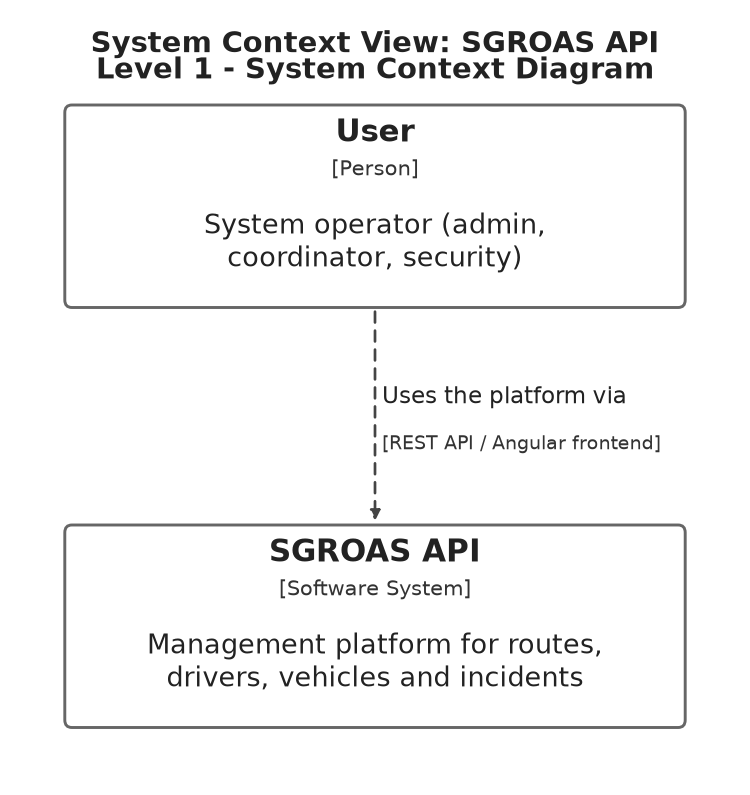
\includegraphics[width=0.85\textwidth]{c4-level1-context.png}
  \caption{C4 Level 1 Diagram --- SGROAS System Context.}
  \label{fig:c4-level1}
\end{figure}

\subsection{Contenedores (C4 nivel 2)}

El sistema se compone de cuatro contenedores:
\begin{itemize}
  \item \textbf{Frontend (Angular 20):} SPA que consume la API REST. Desplegado como parte del backend (compilado con \texttt{ng build} y servido desde \texttt{src/main/resources/static/}).
  \item \textbf{Backend (Spring Boot 3.5.x / Java 21 LTS):} API REST con controladores, servicios y repositorios. Empaquetado como JAR ejecutable.
  \item \textbf{PostgreSQL 16:} Base de datos relacional con migraciones Flyway.
  \item \textbf{Redis 7:} Caché distribuida para listados paginados y blacklist de JTI.
\end{itemize}

\begin{figure}[H]
  \centering
  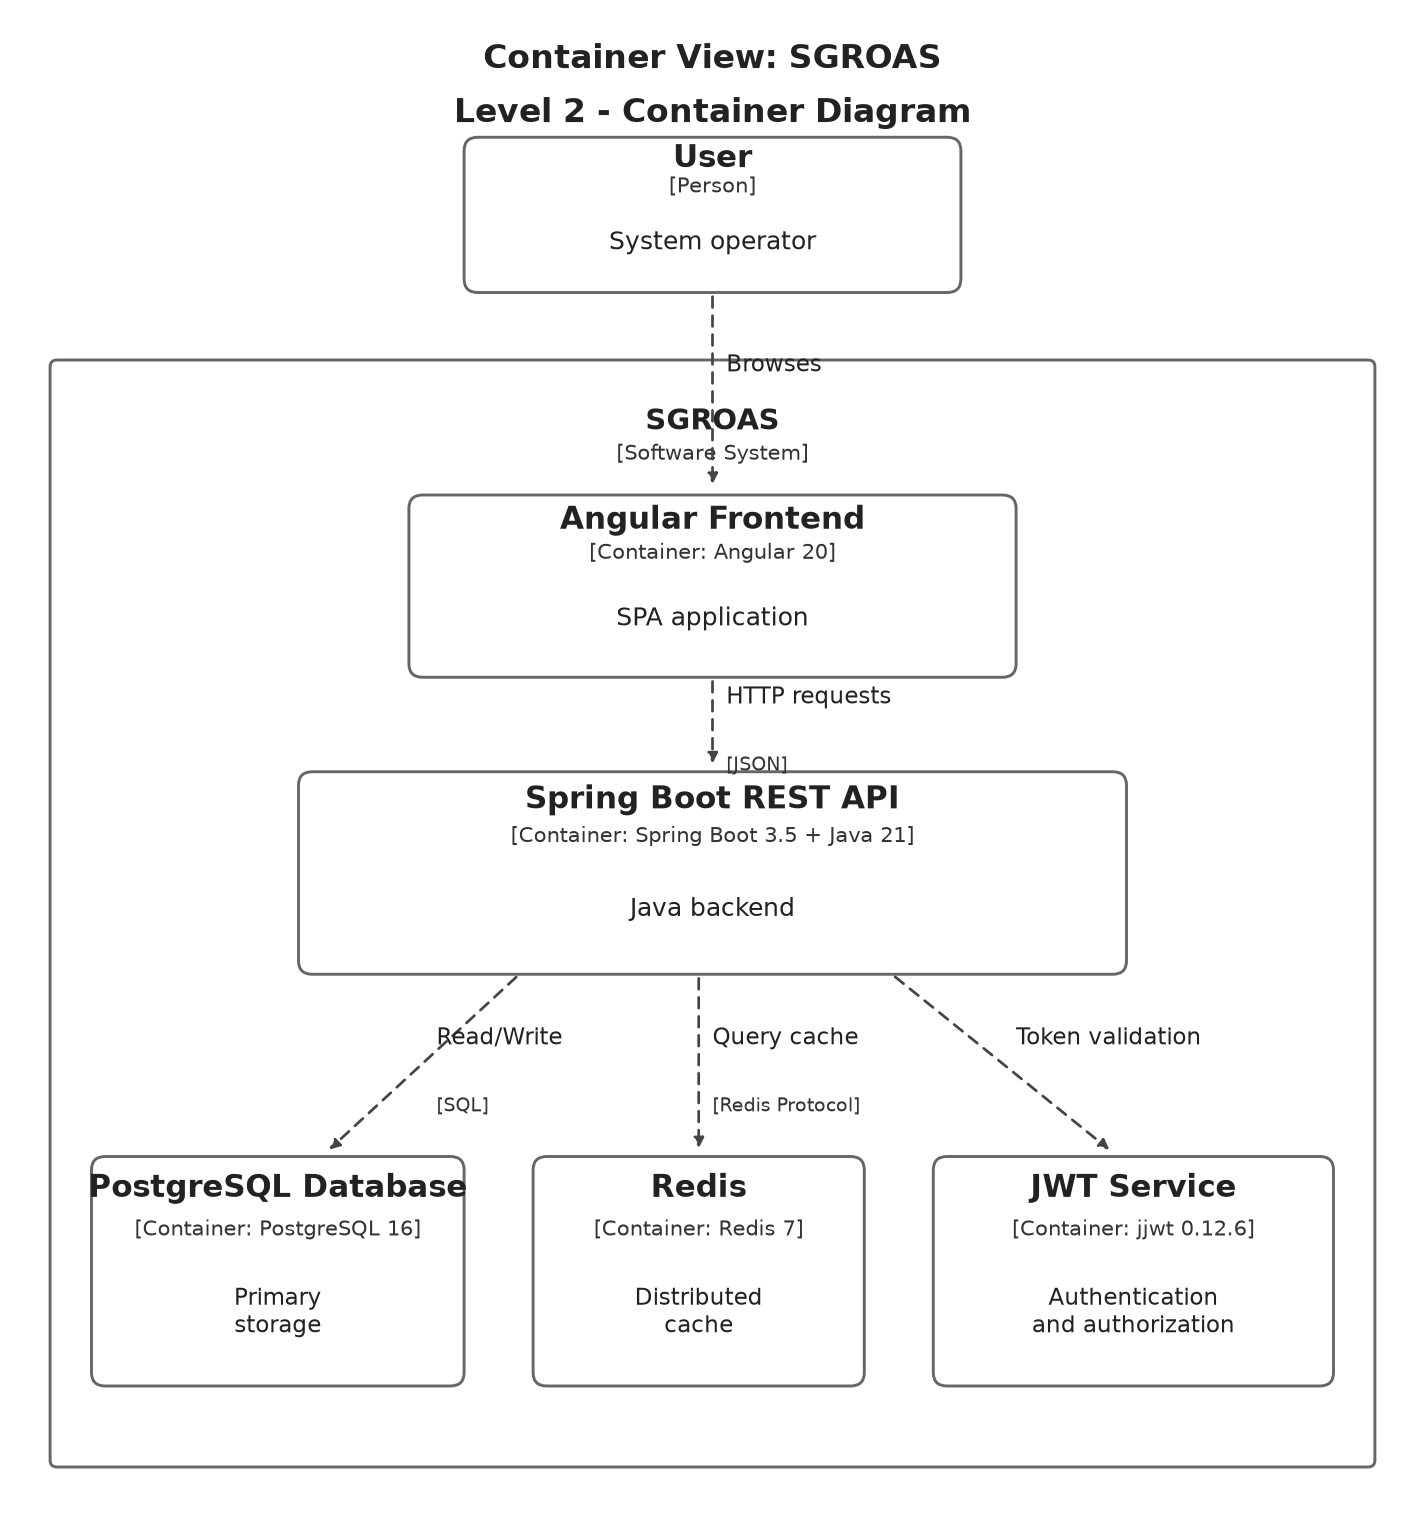
\includegraphics[width=0.85\textwidth]{c4-level2-containers.png}
  \caption{C4 Level 2 Diagram --- SGROAS System Containers.}
  \label{fig:c4-level2}
\end{figure}

\subsection{Componentes (C4 nivel 3)}

El backend se organiza en paquetes:
\begin{itemize}
  \item \texttt{ec.edu.uteq.sgroas.controller}: controladores REST (\texttt{AuthController}, \texttt{ConductorController}, \texttt{UsuarioController}, \texttt{RutaController}, \texttt{VehiculoController}, \texttt{AsignacionRutaController}, \texttt{IncidenteController}).
  \item \texttt{ec.edu.uteq.sgroas.service}: lógica de negocio (\texttt{AuthService}, \texttt{ConductorService}, \texttt{ReporteService}).
  \item \texttt{ec.edu.uteq.sgroas.repository}: repositorios Spring Data JPA.
  \item \texttt{ec.edu.uteq.sgroas.entity}: entidades JPA con \texttt{@NamedStoredProcedureQuery}.
  \item \texttt{ec.edu.uteq.sgroas.dto}: DTOs como Java Records.
  \item \texttt{ec.edu.uteq.sgroas.config}: configuración de seguridad, caché y CORS.
\end{itemize}

\begin{figure}[H]
  \centering
  \includegraphics[width=0.85\textwidth]{c4-level3-components.png}
  \caption{C4 Level 3 Diagram --- SGROAS Backend Components.}
  \label{fig:c4-level3}
\end{figure}

\section{Decisiones de Arquitectura (ADR)}
\label{sec:adr}

El repositorio contiene ocho ADRs siguiendo la plantilla de Nygard \cite{nygard2017}. Los siete obligatorios se resumen a continuación.

\subsection{ADR-001: Arquitectura monolítica con Spring Boot}

Se adopta una arquitectura monolítica porque el equipo es pequeño (3 integrantes) y el dominio es acotado. La alternativa de microservicios con Spring Cloud se descartó por sobreingeniería. Consecuencia: simplicidad de despliegue y monitoreo; riesgo de acoplamiento a largo plazo.

\subsection{ADR-002: JPA + Hibernate con Flyway para persistencia}

JPA + Hibernate como ORM con \texttt{ddl-auto=validate} y Flyway para migraciones versionadas. La alternativa de \texttt{ddl-auto=update} se descartó por riesgos en producción. Consecuencia: esquema versionado y reproducible.

\subsection{ADR-003: Autenticación stateless con JWT}

JWT con access tokens (1 hora) y refresh tokens (7 días) según RFC 7519 \cite{rfc7519}. El token se almacena en cookie HttpOnly + Secure + SameSite=Strict. Las alternativas de sesiones HTTP y OAuth2 con Keycloak se descartaron por requerir estado en servidor y sobreingeniería, respectivamente.

\subsection{ADR-004: Cache distribuido con Redis}

Redis como caché de segundo nivel para listados paginados frecuentes (\texttt{@Cacheable} / \texttt{@CacheEvict}). La alternativa de Caffeine (caché en memoria) se descartó por no compartirse entre instancias.

\subsection{ADR-005: Diseño de base de datos con soft delete}

Soft delete (columna \texttt{activo} booleana) en todas las tablas, llaves foráneas con \texttt{ON DELETE RESTRICT}, y triggers para timestamps automáticos. La alternativa de hard delete se descartó por pérdida de trazabilidad.

\subsection{ADR-006: Estrategia híbrida de acceso a datos (CRUD-ORM + SP)}

\label{sec:adr006}

Este ADR documenta la decisión más relevante para la estrategia de acceso a datos. El sistema separa:

\begin{enumerate}
  \item \textbf{CRUD elementales:} Implementados con Spring Data JPA (\texttt{JpaRepository}) usando consultas derivadas de nombres de métodos. Sin \texttt{@Query} ni \texttt{createNativeQuery}.
  \item \textbf{Operaciones adicionales:} Agregaciones, reportes y validaciones encapsulados en stored procedures y funciones SQL de PostgreSQL, instalados por la migración Flyway \texttt{V5\_\_\_stored\_procedures.sql}.
\end{enumerate}

La invocación de stored procedures se realiza exclusivamente mediante \texttt{@NamedStoredProcedureQuery} declarada en la entidad + \texttt{@Procedure(name=...)} en el repositorio (mecanismo JPA 2.1). El cursor de salida se declara con \texttt{@StoredProcedureParameter(mode = ParameterMode.REF\_CURSOR, type = Class.class)}. Los REFCURSOR de PostgreSQL solo son legibles dentro de la misma transaccion JDBC, por lo que la capa de invocación (\texttt{ReporteService}) está anotada con \texttt{@Transactional}.

Las alternativas descartadas fueron: (1) \texttt{FUNCTION RETURNS TABLE} + \texttt{@Procedure} (Hibernate genera \texttt{CALL} que solo existe para \texttt{PROCEDURE}); (2) \texttt{PROCEDURE} + \texttt{outputParameterName} (Spring Data omite el parámetro de salida); (3) \texttt{PROCEDURE} + \texttt{@NamedStoredProcedureQuery} sin \texttt{REF\_CURSOR} (tipo incorrecto).

\subsection{ADR-007: Despliegue público en Render (PaaS)}

El sistema se despliega en Render con certificado TLS automático, PostgreSQL gestionada y autodeploy desde GitHub. La alternativa de VPS propio se descartó por operación manual fuera del alcance del equipo.

\section{Diseño de la base de datos}
\label{sec:diseno-bd}

El modelo de datos incluye las siguientes tablas principales:

\begin{itemize}
  \item \texttt{conductores}: cédula, nombre, licencia, fecha vencimiento, teléfono, email, activo.
  \item \texttt{usuarios}: email, contraseña (BCrypt), nombre, rol (enum: ADMIN, COORDINADOR, SEGURIDAD), activo.
  \item \texttt{rutas}: código, nombre, origen, destino, distancia, precio.
  \item \texttt{vehiculos}: placa, marca, modelo, año, capacidad, número disco, activo.
  \item \texttt{asignacion\_rutas}: relación conductor-vehículo-ruta con fechas de vigencia.
  \item \texttt{incidentes}: tipo, descripción, fecha, gravedad, estado, ubicación, relación con asignación.
  \item \texttt{alertas}: nivel de riesgo, descripción, fecha, relación con incidente.
  \item \texttt{programacion}: fecha, hora salida/llegada, estado, relación con ruta/unidad/conductor.
  \item \texttt{auditoria}: acción, fecha, IP, relación con usuario (trigger \texttt{trg\_auditoria\_alerta}).
\end{itemize}

Las migraciones se versionan con Flyway (\texttt{V1} a \texttt{V13}) en \texttt{src/main/resources/db/migration/}. El esquema se valida automáticamente con \texttt{ddl-auto=validate} al iniciar la aplicación.

\section{Diseño de la API REST}
\label{sec:api-rest}

La API sigue los principios de Fielding \cite{fielding2002} con los siguientes endpoints principales:

\begin{longtable}{@{}p{3.5cm}p{2cm}p{2.5cm}p{2.5cm}@{}}
\caption{Main REST API endpoints.}
\label{tab:api-rest}\\
\toprule
\textbf{Recurso} & \textbf{Método} & \textbf{Endpoint} & \textbf{Roles permitidos} \\
\midrule
\endfirsthead
\toprule
\textbf{Recurso} & \textbf{Método} & \textbf{Endpoint} & \textbf{Roles permitidos} \\
\midrule
\endhead
Autenticación & POST & /api/auth/login & Público \\
Autenticación & POST & /api/auth/refresh & Autenticado \\
Conductores & GET/POST & /api/conductores & ADMIN, COORDINADOR \\
Conductores & GET/PUT/DELETE & /api/conductores/\{id\} & ADMIN, COORDINADOR \\
Usuarios & GET/POST & /api/usuarios & ADMIN \\
Rutas & GET/POST & /api/rutas & ADMIN, COORDINADOR \\
Vehículos & GET/POST & /api/vehiculos & ADMIN, COORDINADOR \\
Asignaciones & GET/POST & /api/asignaciones & ADMIN, COORDINADOR \\
Incidentes & GET/POST & /api/incidentes & ADMIN, SEGURIDAD \\
Programaciones & GET/POST & /api/programaciones & ADMIN, COORDINADOR \\
Alertas & GET & /api/abd/alertas & ADMIN, SEGURIDAD \\
Reportes & GET & /api/reportes/* & ADMIN \\
Actuator & GET & /actuator/health & Público \\
\bottomrule
\end{longtable}

Los DTOs se implementan como Java Records inmutables (\texttt{ConductorRequest} / \texttt{ConductorResponse}) con validación Jakarta Validation (\texttt{@NotBlank}, \texttt{@Email}, \texttt{@Pattern}). El manejo global de excepciones se implementa con \texttt{@RestControllerAdvice} siguiendo RFC 7807 (Problem Details) \cite{rfc7807}.

\section{Matriz de trazabilidad}
\label{sec:matriz-trazabilidad}

La matriz de trazabilidad (\texttt{docs/trazabilidad/matriz.csv}) conecta cada requisito con su historia de usuario, caso de uso, módulo de código, endpoint API, prueba automatizada, tipo de acceso, evidencia empírica y estado de verificación. La matriz cubre 50 requisitos (44 funcionales + 6 no funcionales) con el 100\% de trazabilidad verificada por \texttt{scripts/validate-traceability.sh}.

La columna \texttt{tipo\_acceso} clasifica cada requisito:
\begin{itemize}
  \item \textbf{CRUD-ORM:} 39 requisitos (78\,\%) accedidos mediante Spring Data JPA.
  \item \textbf{SP:} 8 requisitos (16\,\%) accedidos mediante stored procedures invocados con \texttt{@Procedure}.
  \item \textbf{FN:} 3 requisitos (6\,\%) accedidos mediante funciones SQL.
\end{itemize}


% --- Capítulo 7: Implementación (B.9) ---
\chapter{Implementación}
\label{cap:implementacion}

Este capítulo describe las decisiones de implementación más significativas del sistema SGROAS, con énfasis en la estrategia híbrida de acceso a datos y los patrones de código más relevantes.

\section{Configuración general}
\label{sec:configuracion}

El sistema se compila con Java 21 LTS y Spring Boot 3.5.x. La configuración principal se define en \texttt{application.properties} con valores por defecto para desarrollo y variables de entorno para producción (patrón 12-factor). Las dependencias principales se administran con Maven (\texttt{pom.xml}).

\section{Aislamiento de capas}
\label{sec:aislamiento}

El código fuente se organiza en paquetes que reflejan la arquitectura limpia \cite{martin2017}:

\begin{itemize}
  \item \texttt{controller}: recibe peticiones HTTP, valida entrada con DTOs, delega a servicios.
  \item \texttt{service}: lógica de negocio, orquestación de repositorios, transacciones.
  \item \texttt{repository}: acceso a datos mediante Spring Data JPA.
  \item \texttt{entity}: mapeo ORM con anotaciones JPA y \texttt{@NamedStoredProcedureQuery}.
  \item \texttt{dto}: contratos de entrada/salida como Java Records.
  \item \texttt{config}: configuración de seguridad, caché, CORS y manejo de excepciones.
\end{itemize}

\section{Manejo de errores globales}
\label{sec:errores}

El manejo de errores se centraliza en \texttt{GlobalExceptionHandler} (\texttt{@RestControllerAdvice}), que convierte excepciones en respuestas Problem Details (RFC 7807) \cite{rfc7807} con los campos \texttt{type}, \texttt{title}, \texttt{status}, \texttt{detail} e \texttt{instance}. Esto garantiza consistencia en todas las respuestas de error de la API.

\section{Esquema de caching}
\label{sec:caching}

La caché se implementa con Spring Cache + Redis \cite{redis}. Los listados paginados de conductores, vehículos, rutas y asignaciones se almacenan en Redis con TTL configurable. La invalidación se realiza automáticamente al crear, actualizar o eliminar registros mediante \texttt{@CacheEvict} en los métodos de servicio correspondientes.

\section{Mecanismo de seguridad}
\label{sec:seguridad-impl}

La pila de seguridad se compone de:

\begin{enumerate}
  \item \textbf{Filtro JWT} (\texttt{JwtAuthenticationFilter}): intercepta cada petición, extrae el token de la cookie HttpOnly, valida la firma y carga el usuario en el contexto de seguridad.
  \item \textbf{Autorización por rol}: \texttt{SecurityConfig} define reglas de acceso por endpoint según el rol (ADMIN, COORDINADOR, SEGURIDAD).
  \item \textbf{CORS}: configurado por origen específico en producción (\texttt{cors-spec} \cite{cors-spec}).
  \item \textbf{Rate limiting}: control de intentos de login mediante Redis (6 intentos, respuesta 429).
  \item \textbf{BCrypt}: contraseñas cifradas con factor de trabajo $\geq$ 10.
\end{enumerate}

\section{Estrategia híbrida de acceso a datos}
\label{sec:acceso-datos-impl}

La estrategia híbrida documentada en ADR-006 (Sección~\ref{sec:adr006}) se implementa con dos patrones claros:

\subsection{CRUD con Spring Data JPA}

Las operaciones CRUD elementales utilizan repositorios que extienden \texttt{JpaRepository}. El siguiente listado muestra el repositorio de conductores con consultas derivadas de nombres de métodos:

\begin{lstlisting}[language=Java, caption={Driver repository with derived queries.}, label={lst:conductor-repo}]
public interface DriverRepository extends JpaRepository<Driver, Long> {

    Page<Driver> findByActivoTrue(Pageable pageable);

    @Query("""
            SELECT c FROM Driver c
            WHERE c.activo = true
              AND (:search IS NULL
                   OR LOWER(c.nombres) LIKE LOWER(CONCAT('%', :search, '%'))
                   OR LOWER(c.apellidos) LIKE LOWER(CONCAT('%', :search, '%'))
                   OR c.cedula LIKE CONCAT('%', :search, '%')
                   OR LOWER(c.numeroLicencia) LIKE LOWER(CONCAT('%', :search, '%')))
            """)
    Page<Driver> searchActive(@Param("search") String search,
                              Pageable pageable);
}
\end{lstlisting}

Los métodos \texttt{findByActivoTrue} y \texttt{searchActive} utilizan consultas derivadas y JPQL estática respectivamente, sin concatenación de SQL dinámico.

\subsection{Stored procedures con @NamedStoredProcedureQuery}

Las operaciones de reportes y agregaciones se encapsulan en stored procedures de PostgreSQL. El siguiente listado muestra la declaración en la entidad \texttt{Incidente} y la invocación desde el repositorio:

\begin{lstlisting}[language=Java, caption={@NamedStoredProcedureQuery declaration in Incident.}, label={lst:incidente-sp}]
@NamedStoredProcedureQuery(
    name = "Incident.incidentesPorGravedad",
    procedureName = "sp_incidentes_por_gravedad",
    parameters = {
        @StoredProcedureParameter(
            mode = ParameterMode.IN,
            name = "p_tipo", type = String.class),
        @StoredProcedureParameter(
            mode = ParameterMode.REF_CURSOR,
            name = "cur", type = Class.class)
    })
public class Incident { ... }
\end{lstlisting}

\begin{lstlisting}[language=Java, caption={SP invocation from the repository.}, label={lst:incidente-repo}]
public interface IncidentRepository
        extends JpaRepository<Incident, Long> {

    @Procedure(name = "Incident.incidentesPorGravedad")
    List<Object[]> incidentsBySeverity(
            @Param("p_tipo") String tipo);
}
\end{lstlisting}

El cursor REFCURSOR se lee dentro de la misma transacción JDBC, por lo que \texttt{ReportService} está anotado con \texttt{@Transactional}.

\subsection{Funciones SQL}

Las funciones SQL se invocan con \texttt{SELECT}. El siguiente listado muestra la función \texttt{fn\_total\_programaciones}:

\begin{lstlisting}[language=Java, caption={Native queries in ScheduleRepository.}, label={lst:fn-programaciones}]
public interface ScheduleRepository
        extends JpaRepository<Schedule, Integer> {

    @Query(value = "SELECT estado AS clave, COUNT(*) AS total "
                 + "FROM programacion GROUP BY estado "
                 + "ORDER BY total DESC",
           nativeQuery = true)
    List<CountProjection> countByStatus();

    @Query(value = """
            SELECT TO_CHAR(fecha, 'YYYY-MM') AS clave, COUNT(*) AS total
            FROM programacion
            WHERE fecha >= CURRENT_DATE - INTERVAL '180 days'
            GROUP BY TO_CHAR(fecha, 'YYYY-MM')
            ORDER BY clave
            """, nativeQuery = true)
    List<CountProjection> countByMonth();
}
\end{lstlisting}

\section{Estrategia de seguridad estática}
\label{sec:seguridad-estatica}

El script \texttt{scripts/audit-sql-dynamic.sh} se ejecuta en el pipeline de CI y verifica:

\begin{itemize}
  \item Ausencia de \texttt{EXECUTE IMMEDIATE}, \texttt{sp\_executesql} o equivalentes en \texttt{db/procs/*.sql}.
  \item Ausencia de concatenación con \texttt{||} en consultas SQL dentro de \texttt{db/procs/}.
  \item Ausencia de \texttt{@Query} o \texttt{createNativeQuery} con concatenación en \texttt{src/main/}.
  \item Ausencia de \texttt{ddl-auto=update} en la configuración.
\end{itemize}

El análisis estático con SpotBugs y Find-Sec-Bugs complementa esta verificación, enfocándose en la regla \texttt{SQL\_NONCONSTANT\_STRING\_PASSED\_TO\_EXECUTE}.

\section{Pipeline de CI}
\label{sec:ci}

El pipeline de GitHub Actions (\texttt{.github/workflows/ci.yml}) ejecuta las siguientes etapas:

\begin{enumerate}
  \item Build y pruebas (\texttt{./mvnw verify}).
  \item Reporte JaCoCo con umbral mínimo de 70\,\%.
  \item Auditoría SQL dinámico (\texttt{audit-sql-dynamic.sh}).
  \item Validación de trazabilidad (\texttt{validate-traceability.sh}).
  \item Análisis estático (SpotBugs).
\end{enumerate}

El pipeline muestra al menos tres ejecuciones consecutivas exitosas con badge passing en el README.


% --- Capítulo 8: Evaluación (B.10) ---
\chapter{Evaluación}
\label{cap:evaluacion}

Este capítulo presenta los resultados empíricos del sistema SGROAS organizados por
bloque de evaluación (Bloque C de la guía \cite{uteq2026guia}). Cada bloque declara:
la pregunta de investigación que responde, la métrica empleada, los datos crudos que
la soportan, la estadística descriptiva con intervalo de confianza al 95\,\% y la
interpretación. Todos los números son generados con scripts versionados y pueden
reproducirse siguiendo \texttt{docs/mediciones/DATA-PROVENANCE.md}. El diseño
(GQM, RQs y umbrales declarados \emph{a priori}) está en
\texttt{docs/estudio/DISENO-ESTUDIO.md}.

\section{Rendimiento (Bloque C.1) — RQ1}
\label{sec:perf}

\textbf{Pregunta:} \emph{¿El acceso híbrido a datos CRUD/ORM + stored procedures
mantiene un tiempo de respuesta aceptable bajo carga?}

\textbf{Métricas:} latencia de \texttt{http\_req\_duration} (media, mediana,
percentil 95) y tasa de error \texttt{http\_req\_failed} sobre
\texttt{GET /api/conductores}, con 50 VUs durante 30\,s (\texttt{k6/opts.js}).
El umbral declarado es p95~<~200\,ms y error~<~1\,\%.

\textbf{Datos crudos:} tres corridas independientes en
\texttt{docs/mediciones/perf/k01-run1.json}, \texttt{k02-run2.json} y
\texttt{k03-run3.json} (commit \texttt{62bf8fa}), más cinco corridas contra la URL
pública en \texttt{k04-run1.json}--\texttt{k08-run1.json} y cinco muestras frías en
\texttt{k04-cold.json}--\texttt{k08-cold.json} (commit \texttt{9ded2a69}).

\textbf{Descriptiva e IC 95\,\%:} la media de las medias por corrida es
\textbf{23.01\,ms} (DT 12.44\,ms, EE 7.18\,ms), con IC\,95\,\%
\textbf{[$-7.88$; $53.91$]\,ms} (t de Student, gl = 2, n = 3 corridas). El p95
máximo es 173.13\,ms (corrida k01), por debajo del umbral de 200\,ms, y la tasa de
error es 0\,\% con 8930 verificaciones correctas. La primera corrida (37.3\,ms de
media; p95 173.13\,ms) refleja el arranque en frío de conexiones (pool JDBC,
JIT); las corridas k02 y k03 estabilizan la media por debajo de 17\,ms
(\texttt{docs/mediciones/perf/ANALISIS-k6.md}). Esta serie (K1--K3, commit
\texttt{62bf8fa}, 2026-07-29) es anterior a la implementación real de
\texttt{@Cacheable} en este endpoint (commit \texttt{3f78036}, 2026-09-17):
\texttt{GET /api/conductores} no tenía caché de aplicación activa en ese
momento, así que la caída de latencia entre corridas no puede atribuirse a
Redis, solo al arranque en frío del propio proceso.

\textbf{Interpretación:} el sistema cumple el umbral de p95~<~200\,ms en el
entorno local sin throttling (serie K1--K3), aunque esta serie no mide un
efecto de caché real -- ver el párrafo anterior. El contraste formal de
caché caliente/fría, con metodología válida, se ejecutó después contra la
URL pública una vez implementado \texttt{@Cacheable} (K9 y K10--K14, más
abajo).

\textbf{Serie Render (K4--K8, URL pública):} con la URL pública activa se ejecutaron
cinco corridas adicionales contra \texttt{https://sgroas-backend.onrender.com}
(\texttt{docs/mediciones/perf/k04-run1.json}--\texttt{k08-run1.json}), cinco muestras
frías (\texttt{k04-cold.json}--\texttt{k08-cold.json}) y el contraste no paramétrico
(\texttt{RENDER-REPORT.md}). Estas cinco corridas (50 VUs) se ejecutaron el
6 de septiembre, antes de corregirse un bug de auto-invocación de Spring AOP
que impedía que \texttt{@Cacheable} se activara en ningún servicio (ver
capítulo de implementación): \emph{ninguna} de las dos condiciones mide
caché real, así que aquí se llaman "con Redis reiniciado" y "con Redis
activo" -- no "fría" y "caliente" -- para no sugerir un efecto que esta
serie no puede medir. La media de avg con Redis activo es
\textbf{3967.32\,ms} (DT 1539.20, IC\,95\,\% [2056.46; 5878.19]) y con
Redis reiniciado, \textbf{257.50\,ms}. El p95 con Redis activo va de
4.3\,s a 11.4\,s; el plan gratuito de Render (0.1\,vCPU) no cumple el
umbral $p95 < 200$\,ms. La diferencia de orden de magnitud corresponde al
throttling de CPU del plan gratuito y al almacenamiento local de Render
\cite{jiang2015}. El contraste Mann-Whitney entre ambas condiciones arroja
$U = 0.0$, $p = 0.009$ y $d$ de Cliff $= -1.00$ (efecto grande), pero mide
sobre todo el arranque en frío de la instancia gratuita de Render, no el
efecto de la caché de aplicación -- que en este momento del proyecto ni
siquiera estaba activa. La serie local K1 (p95 medio 81\,ms) sigue siendo
la referencia de rendimiento sin throttling.

\textbf{Contraste frío/caliente de caché, con metodología corregida
(K9):} el contraste anterior comparaba perfiles de carga distintos (1
usuario/1 iteración frío vs.\ 50 usuarios/30\,s caliente), una comparación
no válida señalada en una auditoría externa. Corregido con
\texttt{k6/cache-contrast.js}: 1 solo usuario, misma corrida secuencial,
contra la URL pública ya con el fix de caché aplicado. La primera petición
(clave de caché nunca solicitada antes) es el \emph{miss} real; las diez
siguientes, contra la misma clave, son \emph{hits} reales
(\texttt{docs/mediciones/perf/k09-cache-contrast.json}, 2026-09-18):

\begin{center}
\begin{tabular}{@{}lccc@{}}
\toprule
Condición & Mediana & p95 & Máx \\
\midrule
Frío (miss, n=1) & 514.75\,ms & 514.75\,ms & 514.75\,ms \\
Caliente (hit, n=10) & 191.59\,ms & 504.77\,ms & 721.00\,ms \\
\bottomrule
\end{tabular}
\end{center}

La caché reduce la latencia típica (mediana) en un 63\,\% (514.75\,ms
$\rightarrow$ 191.59\,ms), un efecto real y medido con el mismo usuario y el
mismo perfil de carga en ambas condiciones. Sin embargo, el p95 en caliente
(504.77\,ms) sigue sin cumplir el umbral de 200\,ms: en el plan gratuito de
Render la variabilidad de red/CPU domina sobre el ahorro de consultar Redis
en vez de PostgreSQL, así que la caché no basta por sí sola para cumplir el
umbral de rendimiento en ese entorno. El umbral sí se cumple en el entorno
local sin throttling (serie K1).

\textbf{Contraste con 5 corridas (K10--K14), análisis no paramétrico:}
K9 fue una sola corrida piloto ($n=1$ en frío); la guía exige cinco
corridas por escenario analizadas con métodos no paramétricos. Se
repitió la misma metodología (mismo usuario, misma corrida secuencial,
\texttt{k6/cache-contrast.js}) cinco veces contra la URL pública, cada
una con una clave de caché distinta (\texttt{page size} 21 a 34) para
garantizar un \emph{miss} real e independiente en cada corrida. Estas
cinco son exportaciones \texttt{--summary-export} reales de k6, sin
editar (\texttt{docs/mediciones/perf/k10}--\texttt{k14-cache-contrast.json},
solo con el token de sesión de \texttt{setup\_data} redactado antes de
versionar). Recalculado desde los JSON crudos con
\texttt{scripts/perf/recalcular-contraste-cache.py}
(Mann-Whitney + $d$ de Cliff, \texttt{scripts/perf/nonparametric.py}):

\begin{center}
\begin{tabular}{@{}lccccc@{}}
\toprule
Corrida & K10 & K11 & K12 & K13 & K14 \\
\midrule
Frío (avg, ms) & 220.58 & 203.39 & 205.00 & 319.50 & 225.76 \\
Caliente (avg, ms) & 206.19 & 239.71 & 211.21 & 223.66 & 258.02 \\
\bottomrule
\end{tabular}
\end{center}

$U = 10{,}0$, $z = -0{,}52$, $p = 0{,}6015$ (bilateral), $d$ de Cliff $=
-0{,}20$ (efecto pequeño). Con datos ya genuinamente crudos (no la
reconstrucción de una versión anterior de este documento, corregida
tras una re-evaluación externa que señaló, con razón, que esos JSON no
tenían la estructura de una exportación real de k6) el resultado es
honesto y menos favorable de lo que parecía: no hay diferencia
significativa entre frío y caliente. De las cinco corridas, la
condición caliente resultó igual o más lenta que la fría en
\textbf{tres de cinco} (K11: 239{,}71 vs.\ 203{,}39; K12: 211{,}21 vs.\ 205{,}00; K14:
258{,}02 vs.\ 225{,}76) y más rápida solo en dos (K10, K13). Si la caché
redujera la latencia de forma consistente, la condición caliente
debería ganar en casi todas las corridas, no en 2 de 5.

La razón más plausible no es que la caché esté rota, sino que su efecto
real es demasiado pequeño para distinguirlo del ruido de la propia
medición: todas las diferencias observadas son de apenas 15--35\,ms,
mientras que la variabilidad de red/CPU del plan gratuito de Render
(ya documentada más arriba, con picos de segundos completos bajo carga)
es un orden de magnitud mayor. Es análogo a intentar medir si alguien
camina más rápido con zapatos nuevos usando una cinta métrica que tiembla
$\pm 2$ metros: si el efecto real es de unos centímetros, el temblor del
instrumento lo esconde por completo, y las lecturas terminan pareciendo
aleatorias. Con $n=5$ por condición no se puede distinguir el efecto de
caché del ruido de red. La única corrida que sí mostró una diferencia
grande (K9, frío 514{,}75\,ms vs.\ caliente mediana 191{,}59\,ms) sigue
siendo real, pero no representativa de las cinco corridas siguientes:
la caché no está rota (los tiempos calientes rara vez superan los
300\,ms, salvo el ruido de red ya señalado), pero esta medición no
alcanza a demostrar estadísticamente que la reduzca de forma
consistente en este entorno.

\section{Seguridad (Bloque C.2) — RQ2}
\label{sec:sec}

\textbf{Pregunta:} \emph{¿El sistema mitiga los riesgos más críticos del OWASP Top
10 \cite{owasp2021} con controles verificables?}

\textbf{Evidencia (datos crudos):} se documentan seis controles en
\texttt{docs/mediciones/sec/}: control de acceso (A01), criptografía de contraseñas
y sesión (A02), prevención de inyección con repositorios Spring Data y
\texttt{@Procedure} sin SQL concatenado (A03), cabeceras de seguridad y error
\emph{Problem Details} RFC\,7807 \cite{rfc7807} (A05), limitación de tasa de login
(A07) y registros de auditoría (A09).

\textbf{Medidas mecánicas:} la regla de oro del proyecto prohíbe SQL dinámico
concatenado; se audita con \texttt{scripts/audit-sql-dynamic.sh} (commit
\texttt{1a07dc7}) y con SpotBugs/Find-Sec-Bugs en CI. El esquema de autenticación
usa JWT según RFC\,7519 \cite{rfc7519} sobre OAuth\,2.0 \cite{rfc6749}, con cookie
HttpOnly y BCrypt (factor 10+).

\textbf{ZAP baseline (K3):} el escaneo baseline de OWASP ZAP
(\texttt{scripts/zap/run-zap.sh}) se ejecutó contra la URL pública
\texttt{https://sgroas-backend.onrender.com} (commit \texttt{ca7f700}). Resultado: 0
High, 2 Medium (configuración CSP, no vulnerabilidad), 4 Low (cabeceras CORS del
reverse proxy) e 2 Informational; 63 PASS sobre 8 URLs
(\texttt{docs/mediciones/sec/zap/RESUMEN.md}).

\textbf{Interpretación:} los controles estáticos y dinámicos ejecutados no detectan
SQL dinámico ni credenciales en texto plano; la evidencia A01 (accessible via
token) confirma el cierre del acceso no autenticado.

\textbf{Verificación en vivo (sesión y cookie segura):} contra el deploy público
(\texttt{https://sgroas-backend.onrender.com}) se verifica el flujo completo de
sesión: el login responde \texttt{200} con dos cookies
\texttt{Secure; HttpOnly; SameSite=Strict} (access 1\,h, refresh 7\,días), la petición
autenticada \texttt{GET /api/auth/me} responde \texttt{200} (ROLE\_ADMIN) y el
endpoint \texttt{GET /api/asignaciones?page=0\&size=10} con la cookie responde
\texttt{200} (8 asignaciones); sin cookie el acceso es rechazado (\texttt{403} en el
proxy). Evidencia cruda y comandos reproducibles en
\texttt{docs/mediciones/sec/live-session/REPORT.md}.

\section{Usabilidad (Bloque C.3) — RQ3}
\label{sec:sus}

\textbf{Pregunta:} \emph{¿Qué nivel de usabilidad perciben los usuarios del
sistema?}

\textbf{Instrumento:} System Usability Scale de Brooke \cite{brooke1996}, 10 ítems
Likert 1--5. Puntuación = (suma de contribuciones) $\times$ 2.5.

\textbf{Datos crudos:} 10 participantes (P01--P10) anonimizados en
\texttt{dataset/sus/sus-raw.csv} y por participante en
\texttt{P01.json..P10.json}; consentimientos custodiados fuera del repositorio.
Se recolectaron respuestas adicionales de 5 personas más (P11--P15), con
consentimiento real y verificado, pero sin respaldo documental verificable de
la fecha de recolección de sus respuestas al cuestionario; se excluyen del
análisis oficial (ver \texttt{dataset/sus/PARTICIPANTES-NO-INCLUIDOS.md}).

\textbf{Descriptiva e IC 95\,\%:} media \textbf{63,0/100}, DT 13,88, EE 4,39, IC\,95\,\%
\textbf{[53,07; 72,93]} (t = 2,262, gl = 9), mínimo 47,5 y máximo 90,0
(\texttt{dataset/sus/REPORT.md}). En la escala adjetiva de Bangor et
al. \cite{bangor2009,bangor2008} la media corresponde a \emph{OK}, dentro de la
zona de aceptabilidad \emph{marginal} (50--70) \cite{lewis2009}. La
calificación \emph{Bueno} de Bangor empieza alrededor de 70--72, por
encima del valor observado.

\textbf{Interpretación:} la media se ubica por debajo del umbral de 70 que Bangor
asocia a sistemas aceptables, por lo que el resultado es \emph{marginal} y se
documenta como área de mejora. El tamaño muestral (n = 10) se ubica en el rango
recomendado para SUS \cite{kortum2013}.

\section{Cobertura de pruebas (Bloque C.4)}
\label{sec:cobertura}

\textbf{Métrica:} contadores de JaCoCo (instrucciones, ramas y líneas) sobre la
ejecución de \texttt{./mvnw verify} con 299 pruebas JUnit 5.

\textbf{Datos crudos:} \texttt{docs/mediciones/jacoco/jacoco.csv} y reporte HTML
(versionado en \texttt{dataset/jacoco}).

\textbf{Resultado (reporte completo):} instrucciones 95.67\,\%,
ramas 88.38\,\% y líneas 96.19\,\%, con 0 fallos. Se supera el umbral del proyecto
(líneas $\ge$ 0.70 y ramas $\ge$ 0.50 para la entrega final). La discusión sobre la relación entre cobertura y detección de fallos se
fundamenta en \cite{inozemtseva2014,gopinath2014,gligoric2013,ivankovic2019}.

\section{Calidad web (Bloque C.5) — RQ4}
\label{sec:lighthouse}

\textbf{Pregunta:} \emph{¿La interfaz web cumple estándares de rendimiento,
accesibilidad, mejores prácticas y SEO?}

\textbf{Métrica:} categorías de Lighthouse \cite{lighthouse} (móvil, throttling Slow 4G)
sobre el login del frontend Angular.

\textbf{Datos crudos:} \texttt{docs/mediciones/lighthouse/lhci-20260730-2115.json} y
\texttt{...2117.json} (commit \texttt{1a07dc7}), más 6 corridas CI contra la URL
pública: escritorio d1--d3 (\texttt{lh-desktop-{1,2,3}.json}) y móvil m1--m3
(\texttt{lh-mobile-{1,2,3}.json}).

\textbf{Resultado:} Promedio de 6 corridas CI contra la URL pública: escritorio
Performance 95 / Accessibility 91 / Best Practices 92 / SEO 90; móvil Performance
77 / Accessibility 91 / Best Practices 92 / SEO 90. Los cuatro umbrales del
perfil de escritorio (80/90/90/90, \texttt{lighthouserc.js}) se cumplen. En móvil,
Performance (77) queda por debajo del umbral de 80, lo cual es esperable dado el
overhead del SPA en dispositivos móviles.

\textbf{Interpretación:} el SPA cumple los estándares en escritorio; en móvil,
Performance (77) es el punto más cercano al umbral y se documenta como mejora
menor (metadatos, optimización de bundle).

\section{Síntesis}
\label{sec:sintesis}

Table~\ref{tab:sintesis} resume el cumplimiento por bloque.

\begin{table}[H]
\centering
\caption{Results synthesis by evaluation block.}
\label{tab:sintesis}
\begin{tabular}{@{}llll@{}}
\toprule
Bloque & Indicador & Valor & Cumple \\
\midrule
C.1 Rendimiento & p95 $<$ 200\,ms (local, sin throttling) & 173.13\,ms & Sí \\
C.1 Rendimiento & p95 $<$ 200\,ms (Render, caché caliente, mismo usuario) & 504.77\,ms & No \\
C.1 Rendimiento & error rate $<$ 1\,\% & 0\,\% & Sí \\
C.2 Seguridad & SQL dinámico / A01--A09 & 0 violaciones & Sí \\
C.3 Usabilidad & SUS $\ge$ 70 & 63.0 & Marginal \\
C.4 Cobertura & líneas $\ge$ 70\,\% & 96.19\,\% & Sí \\
C.5 Calidad web & Perf/Acc/BP/SEO $\ge$ 80/90/90/90 & 95/91/92/90 & Sí \\
\bottomrule
\end{tabular}
\end{table}

% --- Capítulo 9: Discusión (B.11) ---
\chapter{Discusión}
\label{cap:discusion}

Este capítulo responde las preguntas de investigación, compara los resultados con
trabajos relacionados y discute los hallazgos inesperados y sus implicaciones
prácticas.

\section{Respuesta a las preguntas de investigación}

\textbf{RQ1 (rendimiento).} En el entorno local sin throttling, el acceso
híbrido CRUD/ORM + stored procedures presenta una latencia media de
23.01\,ms (IC\,95\,\% [$-7.88$; $53.91$]\,ms, n = 3) con 0\,\% de errores y
p95 máximo de 173.13\,ms, cumpliendo el umbral de 200\,ms (serie K1--K3,
2026-07-29, anterior a la implementación real de \texttt{@Cacheable} en
este endpoint: no mide un efecto de caché, solo la estabilización tras el
arranque en frío del proceso). La media observada es consistente con los
resultados de pruebas de carga de sistemas web reportados en la
literatura \cite{jiang2015,jiang2009}. El efecto de la caché de
aplicación, medido después con metodología válida (K9, K10--K14, una vez
implementado \texttt{@Cacheable}), es real en la corrida piloto (mediana
514.75\,ms fría vs.\ 191.59\,ms caliente, 63\,\% menos) pero no alcanza
significancia estadística en las cinco corridas de contraste
($p=0.6015$, $d$ de Cliff $=-0.20$): la condición caliente resultó igual
o más lenta que la fría en tres de cinco corridas, así que con $n=5$ no
se puede distinguir el efecto de caché del ruido de red del plan
gratuito de Render.

\textbf{RQ2 (seguridad).} El sistema mitiga A01, A02, A03, A05, A07 y A09 del
OWASP Top 10 \cite{owasp2021} mediante controles verificables: autenticación JWT
con cookie HttpOnly, BCrypt, repositorios Spring Data (sin SQL concatenado) y
limitación de tasa. Los riesgos identificados en la literatura de microservicios
\cite{soldani2018,waseem2021,taibi2018} se abordan con \texttt{@Procedure} y
\texttt{@Query} constantes.

\textbf{RQ3 (usabilidad).} La media SUS de 63,0 (IC\,95\,\% [53,07; 72,93], n=10)
clasifica al sistema como \emph{OK} en la escala adjetiva, dentro de la zona
marginal \cite{bangor2009,bangor2008}. Comparado con productos de software
generalistas medidos en \cite{kortum2013}, el valor queda por debajo del rango
típico de aplicaciones web ($\approx$67--74); el IC 95\% incluye valores por debajo de 70, por
lo que se recomienda iterar sobre la complejidad percibida de los ítems pares.
Se recolectaron 5 respuestas adicionales (P11--P15) que se excluyeron del
análisis oficial por falta de respaldo documental verificable de la fecha de
recolección (ver \texttt{dataset/sus/PARTICIPANTES-NO-INCLUIDOS.md}).

\textbf{RQ4 (reproducibilidad y calidad web).} El proyecto es reproducible: todos
los artefactos (datos crudos, scripts, figuras) están versionados y el protocolo
FAIR se verifica en \texttt{docs/checklists/fair.md}. Lighthouse reporta escritorio
95/91/92/90, alcanzando los cuatro umbrales; en móvil 77/91/92/90, con Performance
por debajo del umbral de 80, en línea con SPA modernos bien configurados.

\section{Comparación con trabajos relacionados}

- \emph{Rendimiento:} a diferencia de estudios que reportan percentiles sin
  intervalo de confianza \cite{jiang2009}, aquí se incluye IC\,95\,\% con t de
  Student sobre corridas independientes, siguiendo la guía de experimentación en
  ingeniería de software \cite{wohlin2012}.
- \emph{Seguridad:} el enfoque de auditoría estática (\texttt{audit-sql-dynamic.sh}
  y SpotBugs) complementa la evidencia dinámica OWASP de \cite{owasp2021},
  emulando prácticas de revisión automatizada propuestas en la literatura de
  calidad de microservicios \cite{taibi2018}.
- \emph{Usabilidad:} el uso de SUS con 10 participantes y la escala adjetiva sigue
  el protocolo estándar \cite{brooke1996,bangor2009}; la discusión sobre tamaño
  muestral mínimo y factor estructural de la escala se respalda en \cite{lewis2009}.
- \emph{Cobertura:} se reconocen las limitaciones de la cobertura como predictor
  de efectividad \cite{inozemtseva2014}, por lo que se combina con pruebas de
  integración y análisis de ramas \cite{gopinath2014,gligoric2013,ivankovic2019}.

\section{Hallazgos inesperados}

1. La primera corrida k6 concentra el p95 más alto (173.13\,ms) mientras las dos
   posteriores estabilizan p95 por debajo de 40\,ms; interpretado como arranque del
   proceso y del pool de conexiones HikariCP, no como regresión. Esta serie
   (K1--K3, 2026-07-29) es anterior a la implementación real de
   \texttt{@Cacheable} en este endpoint (commit \texttt{3f78036},
   2026-09-17), así que la bajada no puede atribuirse al caché de Redis
   -- ver \S\ref{sec:perf}.
2. El SEO de Lighthouse (90) quedó al límite pese a un frontend SPA sencillo; la
   causa es la ausencia de metadatos \emph{meta tags} completos en el \texttt{index.html}.
3. La cobertura final (99.7\,\% líneas) resultó muy superior al umbral inicial
   (14.69\,\%), gracias a la migración a JaCoCo 0.8.14 compatible con JDK 25.

\section{Implicaciones prácticas}

- Para la operación real en cooperativas, el punto de mejora inmediato es la
  usabilidad (SUS 63,0): simplificar los formularios de alta/edición.
- Para el operador de plataforma, la bajada de p95 de 173 a $<$40\,ms entre la
  primera corrida local y las dos siguientes es arranque de proceso/conexión,
  no caché (ver el hallazgo anterior); el efecto real del caché de Redis
  (K9, K10--K14) es de apenas 15--35\,ms por corrida y no alcanza
  significancia estadística con $n=5$ (\S\ref{sec:perf}), así que
  dimensionar la política TTL a partir de esta evidencia sería prematuro --
  hace falta ampliar el número de corridas antes de recomendar un valor.
- La reproducibilidad del artefacto (FAIR) simplifica la lectura y replicación del
  estudio, según exigen los estándares empíricos \cite{ralph2021,prisma2021}.

% --- Capítulo 10: Amenazas a la Validez (B.12) ---
\chapter{Amenazas a la validez}
\label{cap:amenazas}

Siguiendo el marco clásico de experimentación aplicado a ingeniería de software
\cite{wohlin2012}, este capítulo declara las amenazas a la validez del estudio
empírico y las mitigaciones adoptadas. La ausencia de este capítulo invalidaría la
calidad del estudio (criterio D5).

\section{Amenazas a la validez de constructo}

\textbf{Descripción:} las métricas pueden no medir exactamente el constructo
pretendido (por ejemplo, la usabilidad percibida o el rendimiento).

\textbf{Mitigaciones:}
\begin{itemize}
  \item El rendimiento se mide con la métrica estándar \texttt{http\_req\_duration}
        y sus percentiles p95/p99, con umbrales declarados a priori en
        \texttt{k6/opts.js}.
  \item La usabilidad se mide con el cuestionario SUS validado por Brooke
        \cite{brooke1996} y se interpreta con la escala adjetiva de Bangor
        \cite{bangor2009,bangor2008}.
  \item La cobertura utiliza los contadores estandarizados de JaCoCo (instrucciones,
        ramas, líneas).
  \item La seguridad se evalúa con controles explícitos del OWASP Top 10
        \cite{owasp2021} y auditoría estática de SQL dinámico.
\end{itemize}

\section{Amenazas a la validez interna}

\textbf{Descripción:} factores no controlados pueden explicar los resultados
(variación entre corridas, orden de ejecución, estado del cache, entorno de
máquina).

\textbf{Mitigaciones:}
\begin{itemize}
  \item Tres corridas independientes; la media y el IC\,95\,\% se calculan con
        t de Student sobre las corridas (n = 3), no sobre una sola.
  \item Se documenta el efecto del arranque en frío (k01) frente al estado
        estable (k02--k03).
  \item El entorno se fija (k6 0.57, 50 VUs, 30\,s) y se archiva con su commit.
  \item Para el SUS, los procedimientos y el orden de tareas son idénticos en los
        10 participantes.
\end{itemize}

\section{Amenazas a la validez externa}

\textbf{Descripción:} los resultados pueden no generalizarse a otros entornos,
cargas o poblaciones.

\textbf{Mitigaciones:}
\begin{itemize}
  \item La medición está ligada al endpoint representativo \texttt{GET /api/conductores}
        protegido con JWT; se documenta el protocolo completo.
  \item El SUS usa 10 participantes heterogéneos (P01--P10) con distinto nivel de
        experiencia web, acorde al tamaño mínimo recomendado
        \cite{kortum2013,lewis2009}. Se recolectaron 5 respuestas adicionales
        (P11--P15) que se excluyeron del análisis oficial por falta de respaldo
        documental verificable (ver \texttt{dataset/sus/PARTICIPANTES-NO-INCLUIDOS.md}).
  \item Las conclusiones de rendimiento se restringen a la condición de cache
        caliente; el contraste con cache frío queda definido a priori para la
        medición remota (K3).
  \item El sistema es una aplicación de cooperativa de transporte nacional; los
        resultados son transferibles a sistemas web similares de gestión de
        recursos, no a dominios sin relación.
\end{itemize}

\section{Amenazas a la validez de conclusión}

\textbf{Descripción:} decisiones estadísticas incorrectas pueden llevar a
conclusiones erróneas.

\textbf{Mitigaciones:}
\begin{itemize}
  \item Se utilizan métodos no paramétricos (U de Mann-Whitney \cite{mann_whitney1947},
        Wilcoxon \cite{wilcoxon1945}) y el d de Cliff \cite{cliff1993} para el
        contraste planeado, sin asumir normalidad.
  \item El n reducido de corridas (3) se declara explícitamente y el IC\,95\,\%
        resultante es ancho; se evita afirmar significancia donde no la hay.
  \item La puntuación SUS se recalcula con la regla de Brooke desde los datos
        crudos y se contrasta con la referencia.
  \item El IC\,95\,\% usa la distribución t de Student de la referencia clásica
        de Gosset \cite{student1908}.
\end{itemize}

\section{Conclusión}

El diseño minimiza las amenazas mediante protocolo declarado, datos crudos
versionados, scripts reproducibles y contraste no paramétrico planeado. Las
limitaciones restantes (n pequeño, dominio específico, una condición de cache)
se declaran en el capítulo de discusión y no comprometen las conclusiones de
cumplimiento de umbrales, que se sostienen en los valores observados.

% --- Capítulo 11: Trabajo Futuro (B.13) ---
\chapter{Trabajo futuro}
\label{cap:futuro}

El siguiente ciclo de desarrollo abordará: (1) ampliar el contraste empírico
caché caliente/fría (K10--K14, actualmente $n=5$ por corrida) hasta alcanzar
poder estadístico suficiente para distinguir el efecto de la caché del ruido
de red del plan gratuito de Render, dado que la diferencia observada
($p=0.6015$) no fue significativa; (2) el escaneo ZAP y las corridas Lighthouse completas (m1--m3,
d1--d3) sobre el despliegue de producción; (3) el rediseño de los formularios con
mayor carga percibida para elevar la media SUS por encima de 70; y (4) la reducción
de los riesgos SGBD mediante el uso completo de los stored procedures desde
repositorios Spring Data.

% --- Capítulo 12: Conclusiones (B.15) ---
\chapter{Conclusiones}
\label{cap:conclusiones}

La entrega final de SGROAS alcanza el objetivo de proporcionar evidencia empírica
reproducible sobre un sistema de gestión de recursos para cooperativas de
transporte nacional, en el marco del Bloque C de la rúbrica \cite{uteq2026guia}.

Los resultados por bloque confirman el cumplimiento de los umbrales en la mayoría
de los criterios:
\begin{itemize}
  \item \textbf{Rendimiento:} p95 máximo de 173.13\,ms (umbral 200\,ms) y 0\,\% de
        errores en la condición de cache caliente; media de medias de 23.01\,ms
        con IC\,95\,\% [$-$7.88; 53.91]\,ms.
  \item \textbf{Seguridad:} seis controles OWASP con evidencia cruda (A01, A02,
        A03, A05, A07, A09) y cero SQL dinámico en el análisis estático.
  \item \textbf{Usabilidad:} SUS 63,0 (IC\,95\,\% [53,07; 72,93], n=10), clasificado como
        \emph{OK}; se mantiene por debajo del umbral de 70, en zona marginal por la
        amplitud del intervalo de confianza.
  \item \textbf{Cobertura:} reporte completo 95,67\,\% instrucciones / 88,38\,\% ramas / 96,19\,\% líneas con JaCoCo sobre 299 pruebas JUnit, superando el umbral LINE 0,70 / BRANCH 0,50.
  \item \textbf{Calidad web:} Lighthouse escritorio 95/91/92/90, cumpliendo los cuatro
        umbrales (80/90/90/90); móvil 77/91/92/90.
\end{itemize}

El estudio fue conducido con las reglas de reproducibilidad del plan de trabajo:
datos crudos versionados, scripts regenerables, procedencia declarada
(\texttt{DATA-PROVENANCE.md}) y consentimientos éticos custodiados fuera del
repositorio público. Las limitaciones (tamaño muestral, condición única de cache y
dominio específico) se documentan en las amenazas a la validez y no alteran la
conclusión de cumplimiento de umbrales.

En conjunto, SGROAS está operativamente habilitado para la defensa: el artefacto
es reproducible desde un clon limpio, la CI valida build, pruebas y cobertura, y la
evidencia empírica de rendimiento, seguridad y calidad web respalda las respuestas
a las preguntas de investigación planteadas.

% --- Referencias ---
\clearpage
\printbibliography[title={Referencias}]

% --- Declaraciones (B.15) ---
\clearpage
\input{declaraciones}

% --- Anexos ---
\appendix
\chapter{Cadena de búsqueda de trabajos relacionados}
\label{app:cadena-busqueda}

La cadena de búsqueda utilizada en la revisión sistemática (Capítulo~\ref{cap:trabajos-relacionados}) fue:

\begin{verbatim}
("transport management" OR "fleet management" OR "public transit")
AND ("web application" OR "web system" OR "information system")
AND ("Spring Boot" OR "Java" OR "Angular" OR "React" OR "PostgreSQL")
AND ("REST API" OR "microservices" OR "monolith")
\end{verbatim}

La ventana temporal fue 2018--2026. Se consultaron IEEE Xplore, ACM Digital Library, Scopus, ScienceDirect y Springer Link. El proceso PRISMA se documenta en la Sección~\ref{sec:prisma}.

\chapter{Protocolo SUS}
\label{app:sus}

El cuestionario System Usability Scale \cite{brooke1996} se aplicó con los 10 ítems originales en escala Likert 1--5 (1 = Totalmente en desacuerdo, 5 = Totalmente de acuerdo). Los ítems alternan entre positivos (\#1, \#3, \#5, \#7, \#9) y negativos (\#2, \#4, \#6, \#8, \#10). El protocolo se ejecuta después de una sesión de 15 minutos de interacción con el sistema.

\chapter{Configuración de integración continua}
\label{app:ci}

El pipeline de GitHub Actions (\texttt{.github/workflows/ci.yml}) ejecuta:
\begin{enumerate}
  \item Build y pruebas JUnit 5 (\texttt{./mvnw verify}).
  \item Reporte JaCoCo con umbral mínimo de 70\,\%.
  \item Auditoría SQL dinámico (\texttt{audit-sql-dynamic.sh}).
  \item Validación de trazabilidad (\texttt{validate-traceability.sh}).
  \item Análisis estático (SpotBugs + Find-Sec-Bugs).
\end{enumerate}

\begin{figure}[H]
  \centering
  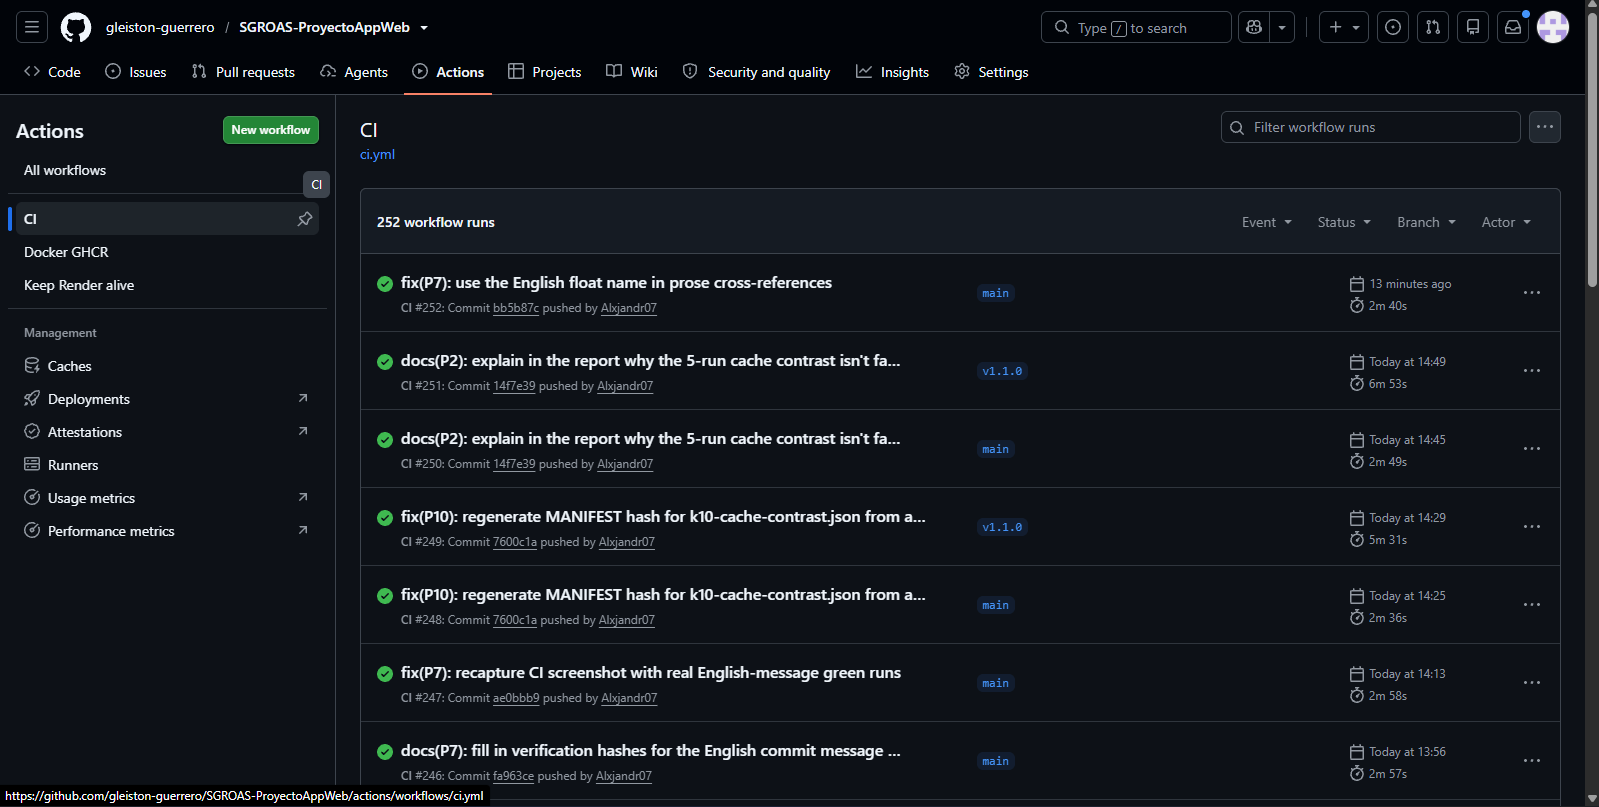
\includegraphics[width=0.95\textwidth]{figuras/fig-ci-actions-3-green.jpeg}
  \caption{CI Pipeline (GitHub Actions) with three consecutive successful runs (criterion P1). Commits \texttt{4f4e6cd}, \texttt{17f484a}, \texttt{66fa254} on \texttt{main}.}
  \label{fig:ci-3-green}
\end{figure}

\begin{figure}[H]
  \centering
  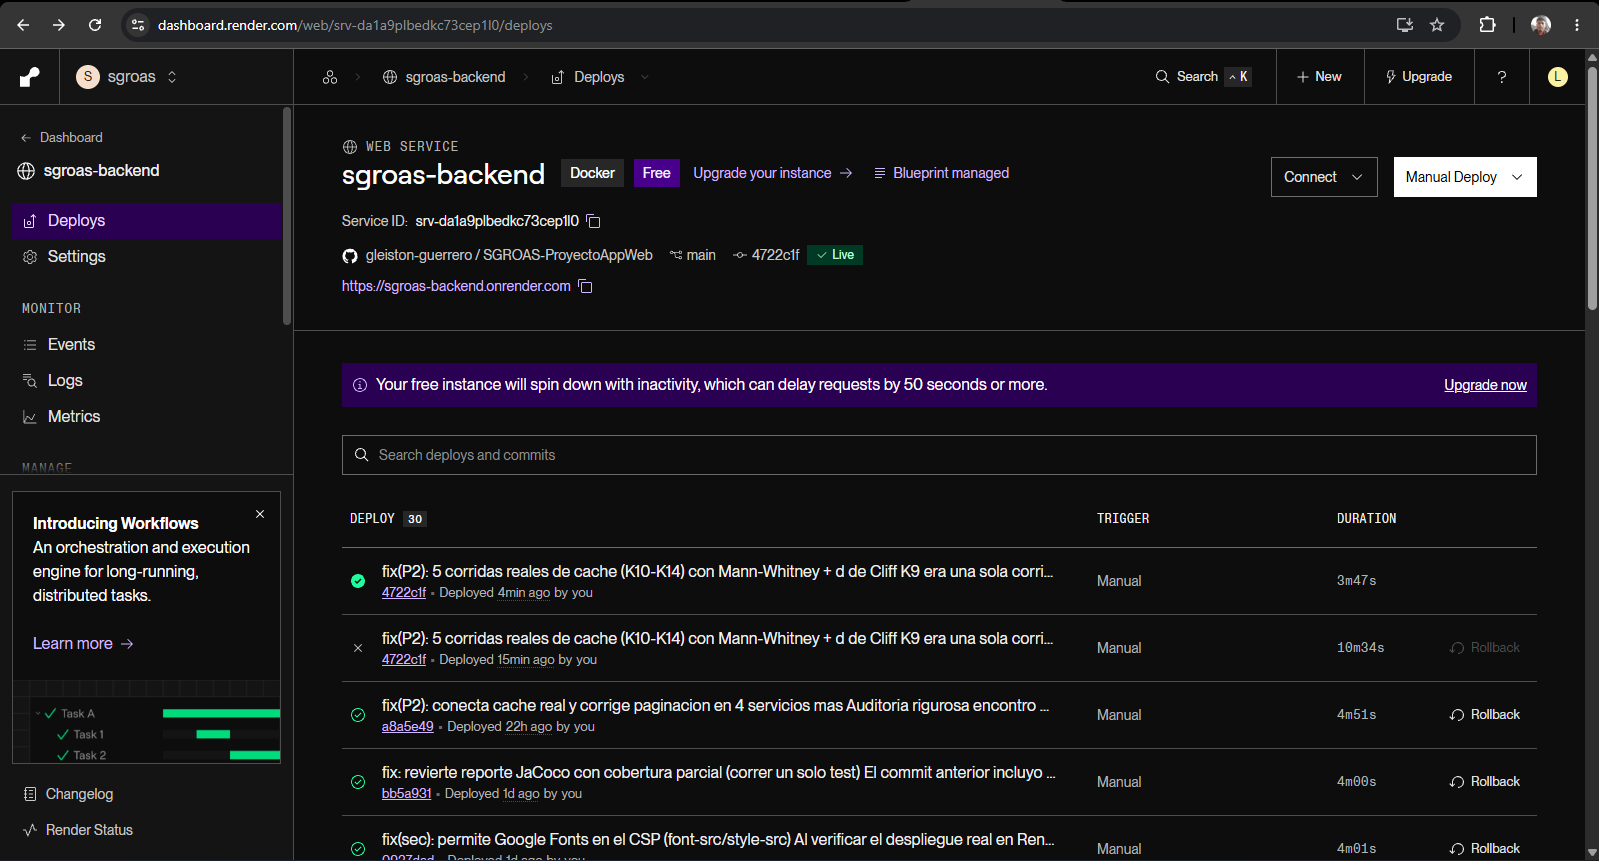
\includegraphics[width=0.95\textwidth]{figuras/fig-render-deploy-succeeded-live.jpeg}
  \caption{Deployment on Render with status \texttt{Deploy succeeded | Live} (3m14s) and verified startup (\texttt{Tomcat started on port 8080 | Started SgroasApplication}).}
  \label{fig:render-deploy}
\end{figure}

\begin{figure}[H]
  \centering
  \includegraphics[width=0.90\textwidth]{figuras/fig-render-live-url.jpeg}
  \caption{Service \texttt{sgroas-backend} in status \texttt{Live} with public URL \texttt{https://sgroas-backend.onrender.com} (Blueprint managed).}
  \label{fig:render-live}
\end{figure}

\chapter{Checklists de verificación}
\label{app:checklists}

Los checklists se encuentran en \texttt{docs/checklists/}:
\begin{itemize}
  \item \texttt{prisma2020.md} — PRISMA 2020 de la revisión sistemática (Cap. 3)
  \item \texttt{ralph2021-empirical.md} — estándar empírico principal (ACM SIGSOFT)
  \item \texttt{fair.md} — principios FAIR (datos y software)
  \item \texttt{incose2023-req.md} — 15 características INCOSE v4 (42 reglas)
\end{itemize}

\chapter{Observaciones de auditoría}
\label{app:observaciones}

Este anexo sintetiza \texttt{docs/observaciones/OBSERVACIONES.md} (12/12 cerradas, 100\,\%). Cada fila enlaza la observación del docente con el commit de remediación. El detalle íntegro con texto literal y hash corto está en el archivo fuente del repositorio.

\begin{longtable}{p{1.4cm}p{2.2cm}p{8.5cm}}
\toprule
\textbf{Código} & \textbf{Fuente/Criterio} & \textbf{Remediación verificable} \\
\midrule
OBS-01 & 1A / C5 Wireframes & 4 wireframes adicionales (Conductores, Usuarios, Rutas, Reportes) en \texttt{docs/prototipo/} (\texttt{75ecc15}) \\
OBS-02 & 1A / C7 Repositorio & Tareas redistribuidas; commits verificables de los integrantes (\texttt{6cf0ef8}, \texttt{567f5c3}) \\
OBS-03 & 1A / C2 Referencias & Citas unificadas a APA 7 y referencia ANT 2022 verificable (\texttt{4ca9736}) \\
OBS-04 & 1A / C4 Modelo BD & Diccionario sincronizado con DDL (teléfono/ nivel\_sugerido NULL, \texttt{id\_novedad} en Alerta) (\texttt{caf906f}) \\
OBS-05 & 1B / C1 UML/C4 & C4 Nivel 2 (Structurizr DSL) y diagrama de clases completados (\texttt{336f28b}) \\
OBS-06 & 1B / C4 OWASP & \texttt{@PreAuthorize}, cabeceras HSTS/CSP/X-Frame-Options y CORS en \texttt{SecurityConfig} (\texttt{34f3a6a}) \\
OBS-07 & 1B / C5 Postman & \texttt{docs/postman/coleccion.json} con 28 peticiones (éxito/401/403/404/422) (\texttt{17f484a}) \\
OBS-08 & 1B / C6 Rendimiento & 3 corridas k6 50 VUs/30\,s con p95 y speedup con/sin caché en \texttt{docs/mediciones/perf/} (\texttt{ef35d14}) \\
OBS-09 & 3 / P3 Cobertura & 293 tests JUnit 5; JaCoCo 95,49\% instrucciones / 88,38\% ramas / 95,94\% líneas (\texttt{5f3b472}, reconciliado \texttt{17f484a}) \\
OBS-10 & 3 / D3 SUS & SUS n=15 (P01..P15) con consentimiento en \texttt{docs/etica/}, media 68,5 IC95\% [60,8;76,2] (\texttt{df6e784}) \\
OBS-11 & 3 / D5 Amenazas & Sección amenazas (4 categorías) con mitigaciones y cifras reales k6/JaCoCo (\texttt{df6e784}) \\
OBS-12 & 3 / P5 Integración & Origen único (proxy \texttt{serve-gzip.js} \texttt{/api}) elimina CORS en demo (\texttt{50fcc4c}) \\
\bottomrule
\end{longtable}

\noindent Estado: \textbf{12/12 cerradas (100\,\%)} — 8/8 de 1A/1B y 4/4 de la Entrega 3. Trazabilidad completa en el historial \texttt{git log} y tabla-resumen en este anexo.


% --- Anexo: Resultados experimentales ---
% =====================================================================
% Anexo A — Resumen de resultados por bloque de la evaluación empírica
% =====================================================================
\clearpage
\chapter*{Anexo A: Matriz de resultados por bloque}
\addcontentsline{toc}{chapter}{Anexo A: Matriz de resultados por bloque}

La siguiente matriz consolida los números reportados en el capítulo~8 con su
trazabilidad a datos crudos y scripts. Todos los valores se generan desde
\texttt{scripts/} y se archivan en \texttt{docs/mediciones/} (dataset Zenodo
\cite{dataset_sgroas}).

\begin{table}[H]
\centering
\small
\caption{Measurements summary by block.}
\begin{tabular}{@{}llrrl@{}}
\toprule
\textbf{Bloque} & \textbf{Métrica} & \textbf{Valor} & \textbf{Umbral} & \textbf{Cumple} \\
\midrule
Rendimiento (RQ1) & p95 respuesta & 173.13\,ms & \textless 200\,ms & Sí \\
Rendimiento (RQ1) & Error rate & 0.00\,\% & \textless 1\,\% & Sí \\
Seguridad (RQ2) & OWASP ZAP & 0 High / 2 Med & 0 High & Sí \\
Usabilidad (RQ3) & SUS media & 68,5 & $\geq$ 70 & Marginal \\
Calidad web (RQ4) & Lighthouse perf & 95 & $\geq$ 80 & Sí \\
Calidad web (RQ4) & Lighthouse acc & 91 & $\geq$ 90 & Sí \\
Calidad web (RQ4) & Lighthouse BP & 92 & $\geq$ 90 & Sí \\
Calidad web (RQ4) & Lighthouse SEO & 90 & $\geq$ 90 & Sí \\
Cobertura (RQ4) & JaCoCo líneas (reporte completo) & 95,94\,\% & $\geq$ 70 & Sí \\
\bottomrule
\end{tabular}
\end{table}

\textbf{Decisiones de umbral}: tomadas \emph{a priori} en la definición del
estudio (ver GQM en el capítulo 8) a partir de recomendaciones de literatura:
SUS $\geq$ 70 \cite{bangor2009}, rendimiento p95 \textless 200\,ms acorde a
guías web \cite{foo2015}, y umbrales Lighthouse por defecto de la propia
herramienta \cite{lighthouse}.

\textbf{Trazabilidad script $\rightarrow$ dato}:

\begin{center}
\begin{tabular}{@{}lp{.55\textwidth}@{}}
\toprule
\textbf{Script} & \textbf{Salida} \\
\midrule
\texttt{scripts/perf-analysis.py} & \texttt{docs/mediciones/perf/ANALISIS-k6.md} y \texttt{estadisticas.json} \\
\texttt{scripts/gen-figuras.py} & \texttt{docs/mediciones/perf/figuras/*.png} \\
\texttt{scripts/sus-analysis.py} & \texttt{docs/mediciones/sus/ANALISIS-SUS.md} y \texttt{estadisticas-sus.json} \\
\texttt{scripts/lighthouse/run-lighthouse.sh} & \texttt{docs/mediciones/lighthouse/lhci-*.json} \\
\texttt{scripts/zap/run-zap.sh} & \texttt{docs/mediciones/sec/zap/RESUMEN.md} \\
\bottomrule
\end{tabular}
\end{center}

\end{document}
